\documentclass{article}

\usepackage{booktabs}
\usepackage{graphicx}
\usepackage{tabularx}
\usepackage{longtable}
\usepackage{hyperref}
\usepackage[bottom]{footmisc}
\usepackage{float}
\usepackage{geometry}
\usepackage[tableposition=below]{caption}
\captionsetup[longtable]{skip=1em} 

\usepackage{listings}
\usepackage{xcolor}

\definecolor{codebg}{RGB}{245,245,244}
\definecolor{sqlkeyword}{RGB}{0,102,204}
\definecolor{sqlcomment}{RGB}{0,153,0}
\definecolor{sqlstring}{RGB}{153,0,0}

\lstdefinelanguage{SQL}{
  morekeywords={SELECT,INSERT,UPDATE,DELETE,FROM,WHERE,AND,OR,NOT,IN,IS,NULL,LIKE,CREATE,TRIGGER,BEFORE,AFTER,FOR,EACH,ROW,BEGIN,END,IF,THEN,ELSE,SIGNAL,SET,DECLARE,INTO,JOIN,ON,AS,COUNT},
  sensitive=false,
  morecomment=[l]--,
  morestring=[b]',
}

\lstset{
  language=SQL,
  backgroundcolor=\color{codebg},
  basicstyle=\ttfamily\small,
  keywordstyle=\color{sqlkeyword}\bfseries,
  commentstyle=\color{sqlcomment}\itshape,
  stringstyle=\color{sqlstring},
  showstringspaces=false,
  breaklines=true,
  frame=single,
  rulecolor=\color{gray},
  numbers=left,
  numberstyle=\tiny\color{gray},
  xleftmargin=1.5em,
  framexleftmargin=1.5em,
  frameround=tttt,
  tabsize=2,
}
\title{Gestione servizio di vehicle sharing}

\author{Lorenzo Peronese, Emanuele Argonni}

\begin{document}

\maketitle

\tableofcontents

\newpage

\section{Analisi dei requisiti}

\subsection{Requisiti in linguaggio naturale}

Si intende realizzare una base di dati per la gestione di un servizio di vehicle sharing elettrici, che offre agli utenti la possibilità di noleggiare automobili, biciclette, monopattini e scooter.
Il sistema dovrà gestire tutti gli aspetti relativi al parco veicoli, agli utenti, ai noleggi e alle ricariche.

Per ciascun veicolo, identificato da un codice univoco, si vogliono memorizzare: tipologia (auto, bici, scooter, monopattino), marca, modello, targa, ultima posizione GPS, stato attuale (disponibile, in uso, in ricarica, fuori servizio), numero di posti, livello di carica della batteria, chilometraggio totale, numero di polizza assicurativa, data di scadenza della revisione. Inoltre si desidera tenere traccia degli interventi di manutenzione e revisione, registrando tipo di intervento, data, costo e officina di riparazione.

Per ogni utente registrato al servizio si desidera tracciare: dati anagrafici (nome, cognome, data e luogo di nascita), documento di riconoscimento, numero di telefono, indirizzo email, estremi della patente di guida se necessari (numero, data di scadenza, categoria), metodo di pagamento, storico dei noleggi effettuati, stato del profilo (attivo, bloccato, in fase di verifica), data di registrazione, abbonamenti attivi.

Riguardo alle stazioni di ricarica dei veicoli si vuole rappresentare: posizione GPS, stato corrente (libera, occupata, in manutenzione, fuori servizio) e la tipologia della presa.

Per ogni noleggio, è necessario registrare: ID univoco, ID dell’utente che lo effettua, ID del veicolo utilizzato, data e ora di inizio noleggio, data e ora di fine noleggio, posizione GPS di inizio e fine noleggio, chilometri percorsi, costo totale, esito del pagamento.

Si vuole modellare la struttura tariffaria del servizio con tariffe base a tempo per ciascuna tipologia di veicolo e la possibilità di acquistare abbonamenti flat (giornalieri, settimanali, mensili).

\subsection{Glossario dei termini}

\begin{table}[H]
\centering
\begin{tabularx}{\textwidth}{|p{2.2cm}|X|p{2.6cm}|p{3cm}|}
\hline
\textbf{Termine} & \textbf{Descrizione} & \textbf{Sinonimi} & \textbf{Collegamenti} \\ \hline
Parco veicoli & Insieme dei veicoli facenti parte del servizio & Flotta veicoli & Veicolo \\ \hline
Veicolo & Mezzo di trasporto elettrico gestito dal servizio & Mezzo & Cliente, Noleggio, Manutenzione, Ricarica \\ \hline
Cliente & Persona registrata al servizio di sharing & Utente, Consumatore & Noleggio, Patente, Metodo di pagamento, Abbonamento \\ \hline
Noleggio & Utilizzo di un veicolo per un certo periodo da parte di un cliente & Corsa, Utilizzo & Cliente, Veicolo \\ \hline
Manutenzione & Intervento tecnico effettuato su un veicolo & Riparazione, Intervento & Veicolo, Officina \\ \hline
Centro di ricarica & Luogo dotato di colonnine per la ricarica dei veicoli & - & Stazione di ricarica \\ \hline
Stazione di ricarica & Colonnina dotata di presa per la ricarica di un veicolo & Colonnina di ricarica & Centro di ricarica, Ricarica \\ \hline
Stato utente & Stato attuale del profilo utente (attivo, sospeso, in fase di verifica) & Stato profilo, stato account & Account \\ \hline
Abbonamento & Piano tariffario prepagato (giornaliero, mensile, ecc.) & Pass & Cliente \\ \hline
Tariffa base & Costo del servizio per unità di tempo differenziato per tipologia di veicolo & Prezzo, Costo & Veicolo \\ \hline
Patente di guida & Documento necessario per il noleggio di auto e scooter & - & Cliente \\ \hline
Metodo di pagamento & Dati carta di debito per pagare i noleggi & - & Account \\ \hline
Posizione GPS & Coordinate GPS che indicano la posizione di un veicolo e/o stazione di ricarica & Coordinate GPS & Veicolo, Stazione di ricarica \\ \hline
Stato veicolo & Stato attuale di un veicolo (disponibile, in uso, in ricarica, fuori servizio) & Disponibilità veicolo & Veicolo \\ \hline
Stato stazione & Stato attuale di una stazione di ricarica (libera, occupata, in manutenzione, fuori servizio) & - & Stazione di ricarica \\ \hline
Officina di riparazione & Struttura che effettua manutenzione dei veicoli & Centro assistenza & Manutenzione \\ \hline
\end{tabularx}
\caption{Glossario dei termini}
\label{table_glossario_termini}
\end{table}

\subsection{Eliminazione delle ambiguità}
Si specifica la differenza tra centro di ricarica e stazione di ricarica: 
\begin{itemize}
    \item stazione di ricarica: rappresenta la singola colonnina fisica per la ricarica di un veicolo
    \item centro di ricarica: luogo in cui si trovano dei parcheggi con diverse colonnine raggruppate per la ricarica simultanea di molti veicoli.
\end{itemize}
Inoltre si fa la distinzione tra la manutenzione programmata (revisione) e interventi tecnici dovuti a danni causati ai veicoli.


\subsection{Struttura dei requisiti}
\subsubsection{Frasi di carattere generale}
Si intende realizzare una base di dati per una società che gestisce un servizio di vehicle
sharing elettrici, che offra agli utenti la possibilità di noleggiare automobili,
biciclette, monopattini e scooter. Il sistema dovrà gestire tutti gli aspetti relativi
al parco veicoli, agli utenti, ai noleggi e alle ricariche.

\subsubsection{Frasi relative ai veicoli}
Di ogni veicolo si vogliono conoscere: tipologia, marca, modello, targa, ultima posizione GPS, stato attuale, numero di posti, percentuale della batteria, chilometraggio totale, numero della polizza assicurativa, data di scadenza della revisione.

\subsubsection{Frasi relative ai clienti}
Di ogni cliente si vogliono memorizzare: dati anagrafici (nome, cognome, data e luogo di nascita), numero di telefono, indirizzo email, documento di riconoscimento, estremi della patente di guida se necessari (numero, data di scadenza, categoria),  stato dell'account (attivo, bloccato, in fase di verifica), data di registrazione, metodo di pagamento, tipologia di abbonamento attivo.

\subsubsection{Frasi relative ai noleggi}
Di ogni noleggio si vogliono tracciare: utente che lo ha effettuato, veicolo utilizzato, data e ora di inizio e fine noleggio con le rispettive posizioni GPS, chilometri percorsi, costo totale, esito del pagamento.

\subsubsection{Frasi relative alla stazioni di ricarica}
Per ogni stazione di ricarica si vogliono rappresentare: posizione GPS, stato corrente, tipologia di presa ("type 2", "schuko", "CCS2").

\subsubsection{Frasi relative alle manutenzione}
Si vuole tracciare lo storico di tutte le manutenzioni effettuate sui veicoli suddivise in revisioni, interventi di riparazione. Per ogni manutenzione si vuole registrare: la tipologia di intervento, il veicolo su cui è stato effettuato, la data, il costo e l'officina di riparazione.

\subsection{Specifica operazioni}

\begin{enumerate}
    \item \textbf{Veicolo:} 
    \begin{enumerate}
        \item \textsc{inserimento:} aggiunta di un veicolo alla flotta
        \item \textsc{modifica:} aggiornamento dei dati dello stato del veicolo (percentuale batteria, posizione GPS, km totali, stato attuale)
        \item \textsc{cancellazione:} rimozione di un veicolo dalla flotta
        \item \textsc{ricerca:} visualizzazione dei veicoli disponibili per tipologia con il livello della batteria maggiore del 20%
        \item \textsc{ricerca:} visualizzazione dei 10 veicolo più noleggiati nell'ultimo anno per tipologia
        \item \textsc{ricerca}: visualizzazione dei 5 veicoli che hanno ricevuto più interventi nell'ultimo anno
    \end{enumerate}
    \item \textbf{Noleggio:}
    \begin{enumerate}
        \item \textsc{inserimento:} avvio di un nuovo noleggio da parte di un cliente
        \item \textsc{modifica:} aggiornamento dei dati (km percorsi, costo, durata, esito pagamento) alla conclusione del noleggio
        \item \textsc{ricerca:} visualizzazione della durata media dei noleggi per ogni tipologia
        \item \textsc{ricerca:}: visualizzazione dei veicoli con più chilometri percorsi nei noleggi
        \item \textsc{ricerca.}: visualizzazione andamento mensile dei noleggi
    \end{enumerate}
    \item \textbf{Cliente:}
    \begin{enumerate}
        \item \textsc{inserimento:} registrazione di un nuovo utente al servizio
        \item \textsc{modifica:}: aggiunta degli estremi della patente di guida
        \item \textsc{cancellazione:} rimozione dell'account di un utente
        \item \textsc{ricerca:} visualizzazione dei clienti con più di 50 noleggi nell'ultimo anno
        \item \textsc{ricerca:} visualizzazione dei clienti con abbonamento in corso di validità
        \item \textsc{ricerca:} visualizzazione dei 10 clienti registrati da più tempo al servizio
    \end{enumerate}
    \item \textbf{Manutenzioni:}
    \begin{enumerate}
        \item \textsc{inserimento:} registrazione di un intervento tecnico e/o revisione per un veicolo
        \item \textsc{ricerca:} visualizzazione tipologie di intervento più costose in media
        \item \textsc{ricerca:} visualizzazione degli ultimi 5 noleggi (e relativi clienti)  di un veicolo soggetto a intervento di riparazione
        \item \textsc{ricerca:} andamento mensile dei costi degli interventi di riparazione
    \end{enumerate}
    \item \textbf{Ricarica:}
    \begin{enumerate}
        \item \textsc{inserimento:} registrazione inizio di una nuova sessione di ricarica
        \item \textsc{modifica:} aggiornamento dei dati (data, costo, KWh caricati) al termine della sessione
        \item \textsc{ricerca:} visualizzazione dei 10 veicoli che hanno effettuato più ricariche nell'ultimo mese
        \item \textsc{ricerca:} visualizzazione degli operatori che hanno effettuato più ricariche
    \end{enumerate}
    \item \textbf{Centri di ricarica:}
    \begin{enumerate}
        \item \textsc{inserimento:} aggiunta di un nuovo centro di ricarica
        \item \textsc{ricerca:} visualizzazione dei centri di ricarica ordinati per energia totale erogata
        \item \textsc{ricerca:} visualizzazione dei 5 centri di ricarica con più ricariche effettuate nell'ultimo anno    
        \item \textsc{ricerca:} Visualizzazione di tutti i centri di ricarica ordinati per numero di colonnine libere
    \end{enumerate}
    \item \textbf{Stazioni di ricarica:}
    \begin{enumerate}
        \item \textsc{inserimento:} aggiunta di una nuova stazione di ricarica
        \item \textsc{modifica:} aggiornamento dello stato della colonnina
        \item  \textsc{ricerca:} visualizzazione delle stazioni ordinate per energia totale erogata
        \item \textsc{ricerca:} visualizzazione della durata media delle sessioni di ricarica per stazione
    \end{enumerate}
    \item \textbf{Tariffa:}
    \begin{enumerate}
        \item \textsc{modifica}: modifica della tariffa di una certa tipologia di veicolo
    \end{enumerate}
\end{enumerate}

\newpage

\section{Progettazione concettuale}

\subsection{Identificazione delle entità e relazioni}

Inizialmente sono state identificate le entità principali del servizio: cliente, operatore ricarica, account, auto, bicicletta, scooter, monopattino, officina, stazioni di ricarica, centro di ricarica, addetto call center, abbonamento, tariffa base.
Abbiamo definito 4 macro gruppi per racchiudere tutte le entità: 
\begin{itemize}
    \item \textbf{Persona}: Generalizzazione di \textsc{cliente}, \textsc{opertore ricarica}, \textsc{addetto call center}.
    \item \textbf{Veicolo}: Fa riferimento a tutte le tipologie di veicoli gestiti dal servizio (\textsc{auto}, \textsc{scooter}, \textsc{monopattini} e \textsc{biciclette}), gli \textsc{abbonamenti} e le \textsc{tariffe} a essi relativi.
    \item \textbf{Ricarica}: Comprende le entità che descrivono l'infrastruttura di ricarica, ovvero \textsc{colonnina di ricarica} e \textsc{centro di ricarica} e l'entità \textsc{Ricarica} che registra le varie sessione di ricarica. 
    \item \textbf{Interventi}: Include le \textsc{officine} che effettuano interventi e revisioni ai veicoli facenti parte del servizio. 
\end{itemize}

\subsection{Un primo scheletro dello schema}

Seguendo la strategia Top-Down, abbiamo costruito una bozza iniziale del nostro schema ER, utilizzando i 4 gruppi appena descritti e definendo le relazioni tra essi.

\begin{figure}[H]
    \centering
    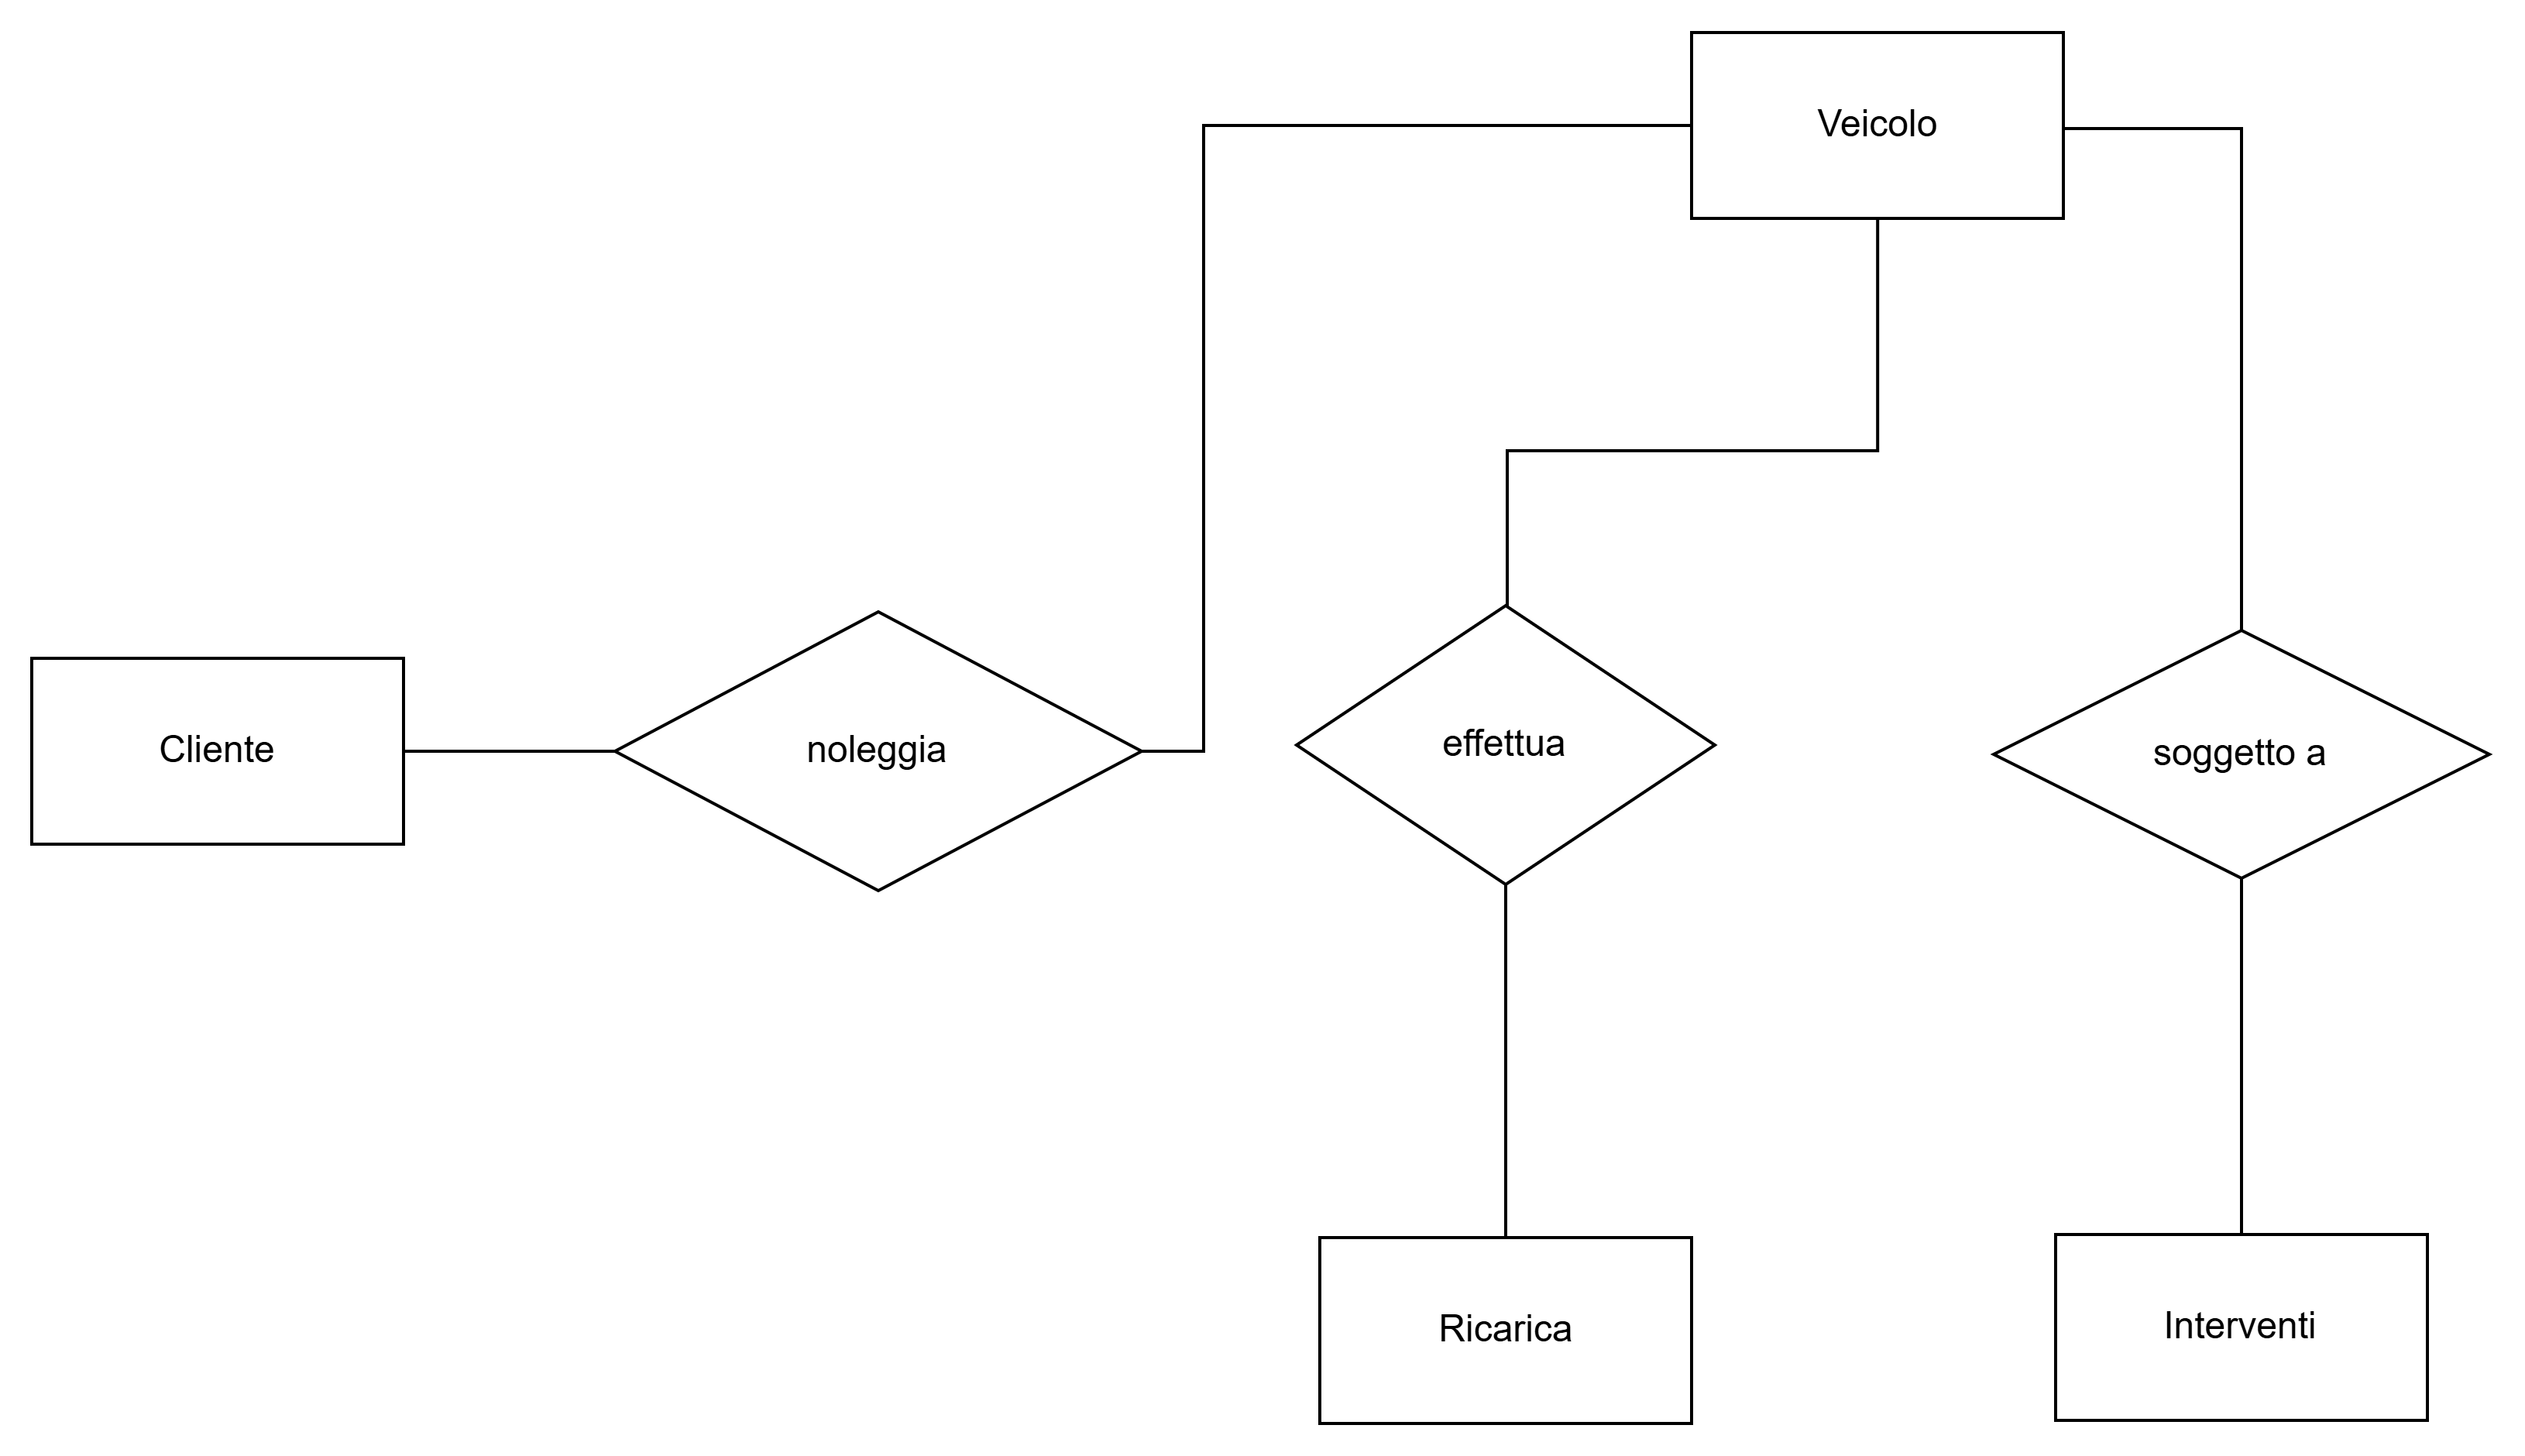
\includegraphics[width=1\linewidth]{top-down.png}
    \caption{Primo scheletro dello schema ER}
    \label{fig:top-down}
\end{figure}


\subsection{Sviluppo delle componenti dello scheletro}

Utilizzando la strategia Bottom-Up, abbiamo utilizzato le entità di base precedentemente definite, suddividendo lo schema ER in sottoschemi più piccoli e concentrandoci sulla costruzione individuale di ognuno di essi.

\subsubsection{Persona}

Abbiamo definito un'entità padre Persona, che comprende tutti gli attributi comuni a Clienti, Operatori ricarica, Addetti call center. Queste entità diventano quindi specializzazioni di Persona, creando un legame di generalizzazione totale disgiunta. Ogni persona che vuole utilizzare il servizio deve registrarsi creando un account personale. Anche il personale possiede un account speciale che permette di fare operazioni non disponibili ai clienti.
I dati patente sono un attributo opzionale, diventano necessari solamente per noleggiare auto e/o scooter.

\begin{figure}[H]
    \centering
    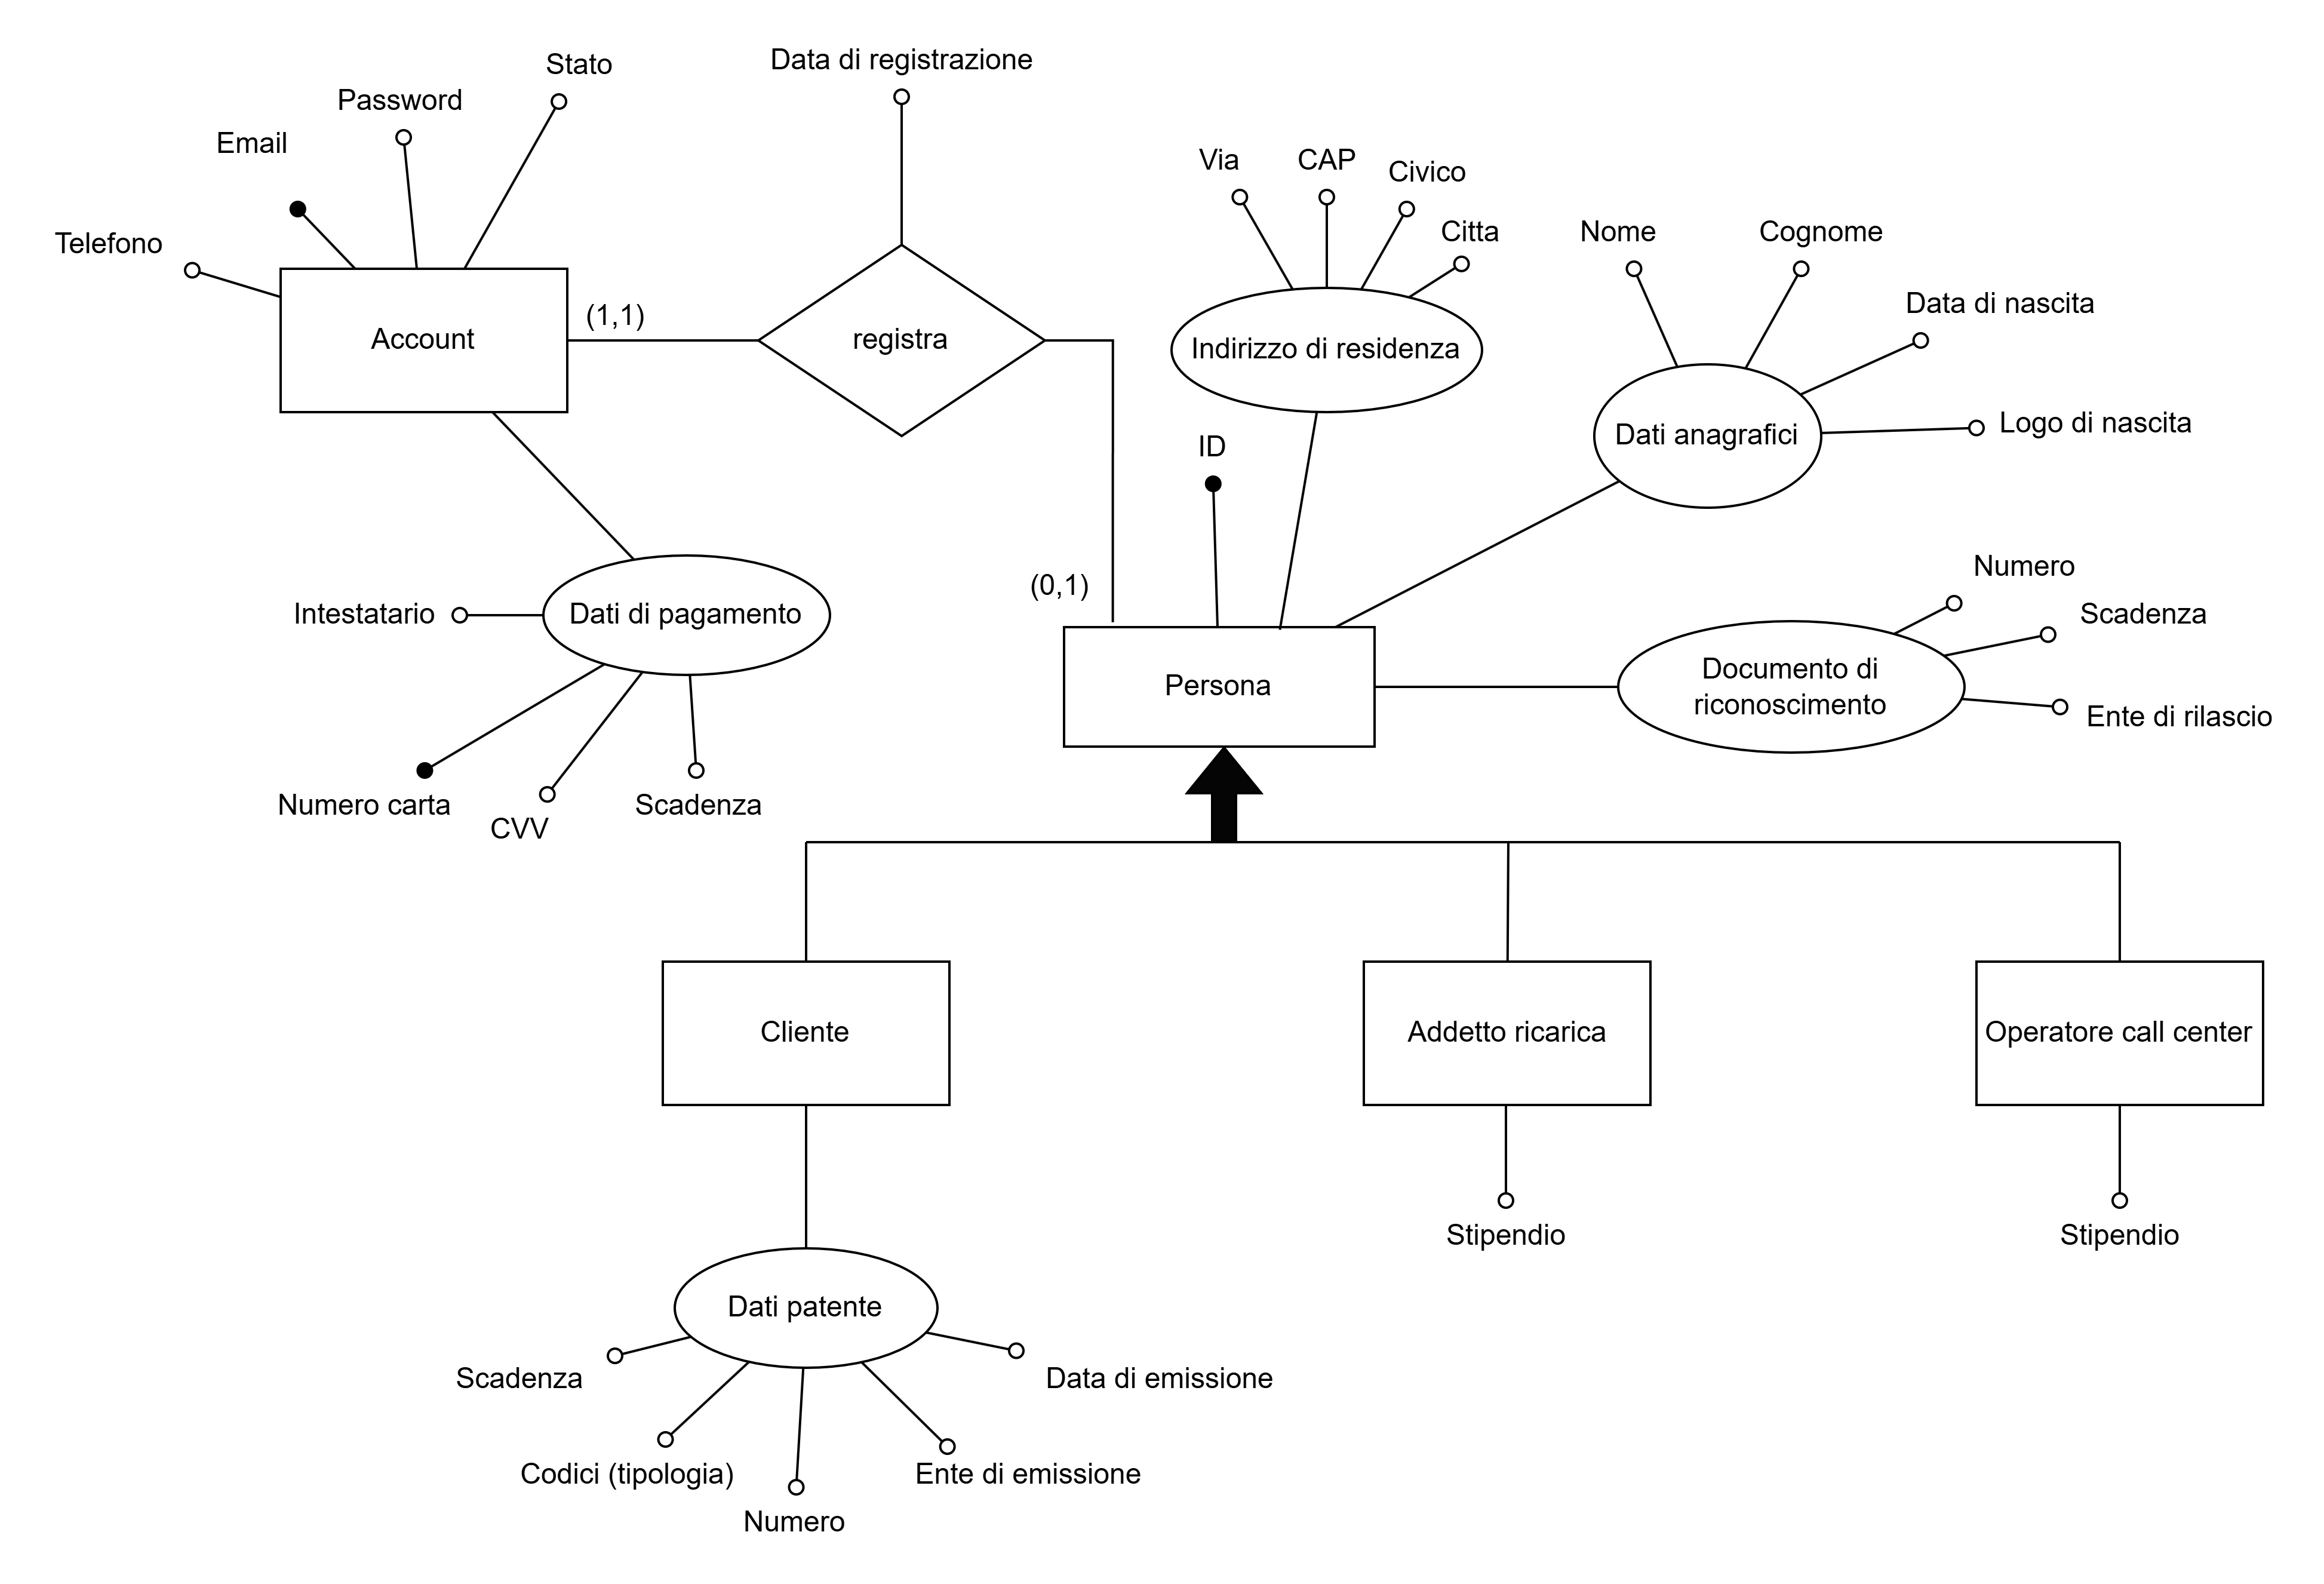
\includegraphics[width=1\linewidth]{bottom-up-persona.png}
    \caption{Schema E.R. clienti, addetti ricarica, operatori call center, account}
    \label{fig:bottom-up-persona}
\end{figure}

\subsubsection{Veicolo}

Le quattro categorie di veicoli (auto, scooter, bici, monopattini) hanno attributi comuni; si è deciso di creare una generalizzazione disgiunta totale definendo l'entità Veicolo. Ogni categoria di veicolo ha una sua tariffa base unitaria (al minuto), è stata quindi creata una relazione "\textsc{veicolo} \textit{soggetto a} \textsc{tariffa}".

\begin{figure}[H]
    \centering
    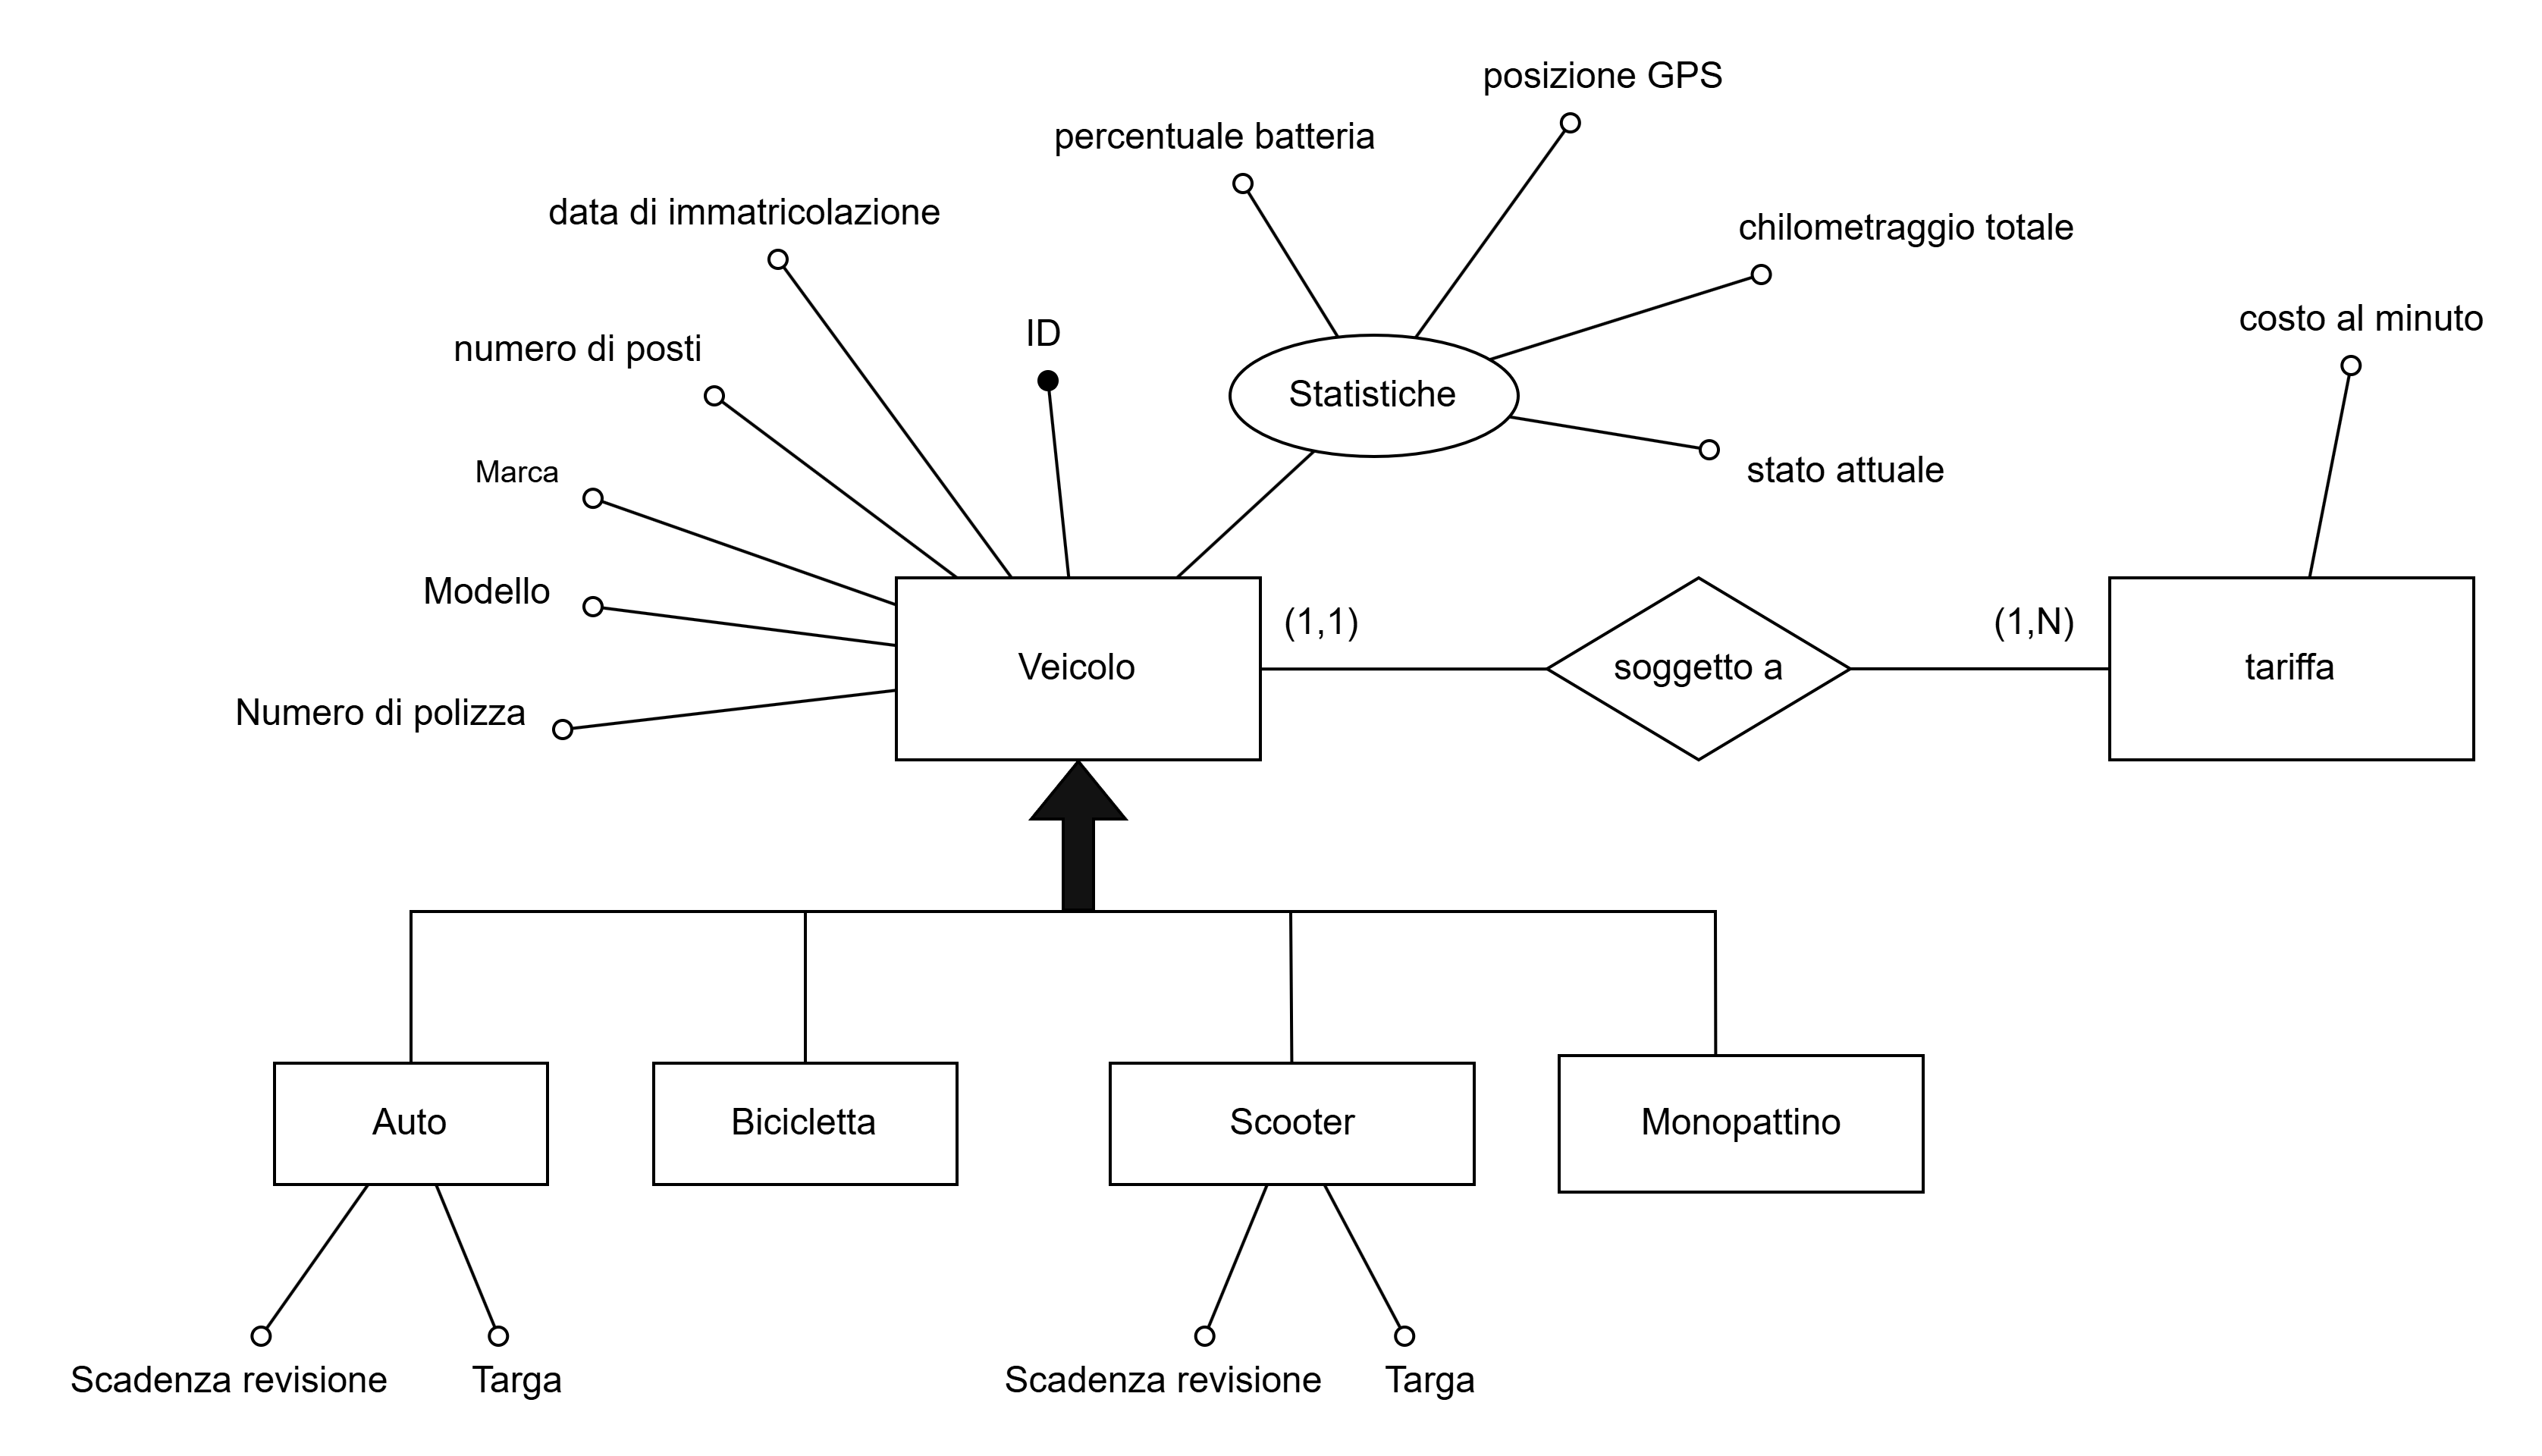
\includegraphics[width=1\linewidth]{bottom-up-veicolo.png}
    \caption{Schema E.R dei veicoli}
    \label{fig:bottom-up-veicolo}
\end{figure}

\subsubsection{Manutenzione}

Ogni veicolo effettua periodicamente la revisione e/o interventi di riparazione presso una delle officine convenzionate; ogni intervento avrà una data, un costo e una tipologia; ogni officina avrà un indirizzo e un recapito telefonico.

\begin{figure}[H]
    \centering
    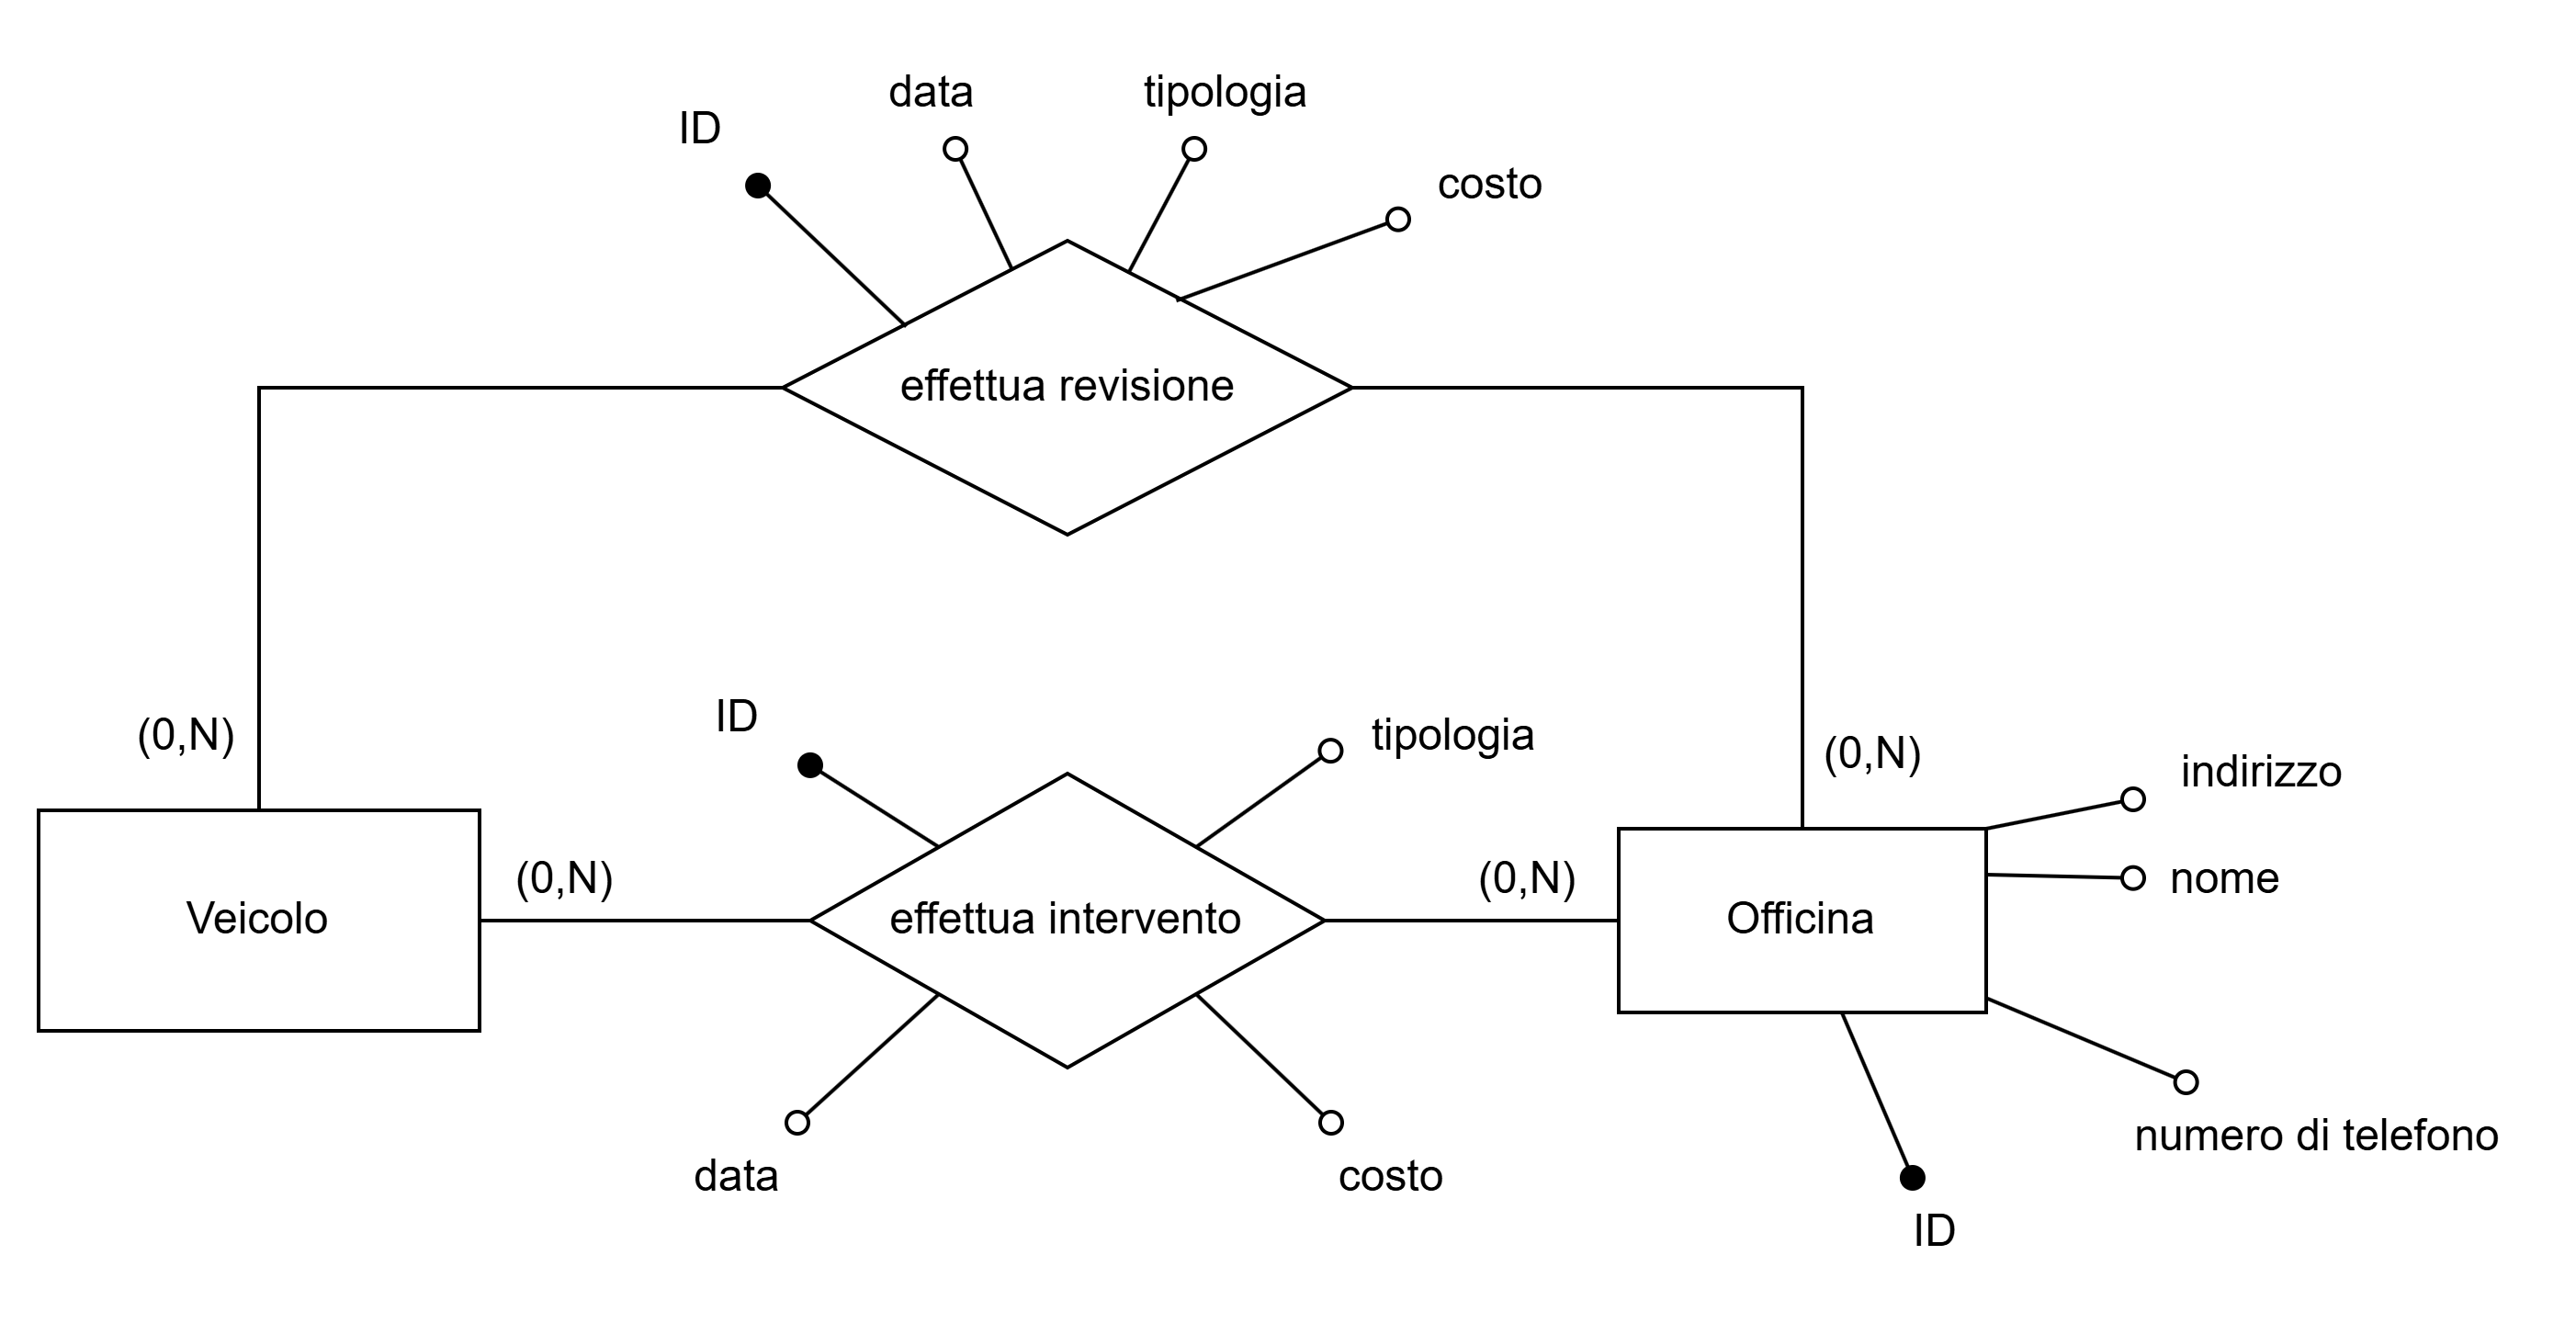
\includegraphics[width=1\linewidth]{bottom-up-manutenzione.png}
    \caption{Schema E.R. delle manutenzioni}
    \label{fig:bottom-up-manutenzioni}
\end{figure}

\subsubsection{Ricarica}

I veicoli vengono ricaricati presso delle stazioni di ricarica, queste possono essere situate (oppure no) in un centro di ricarica; un centro di ricarica è quindi composto da una o più colonnine di ricarica.

\begin{figure}[H]
    \centering
    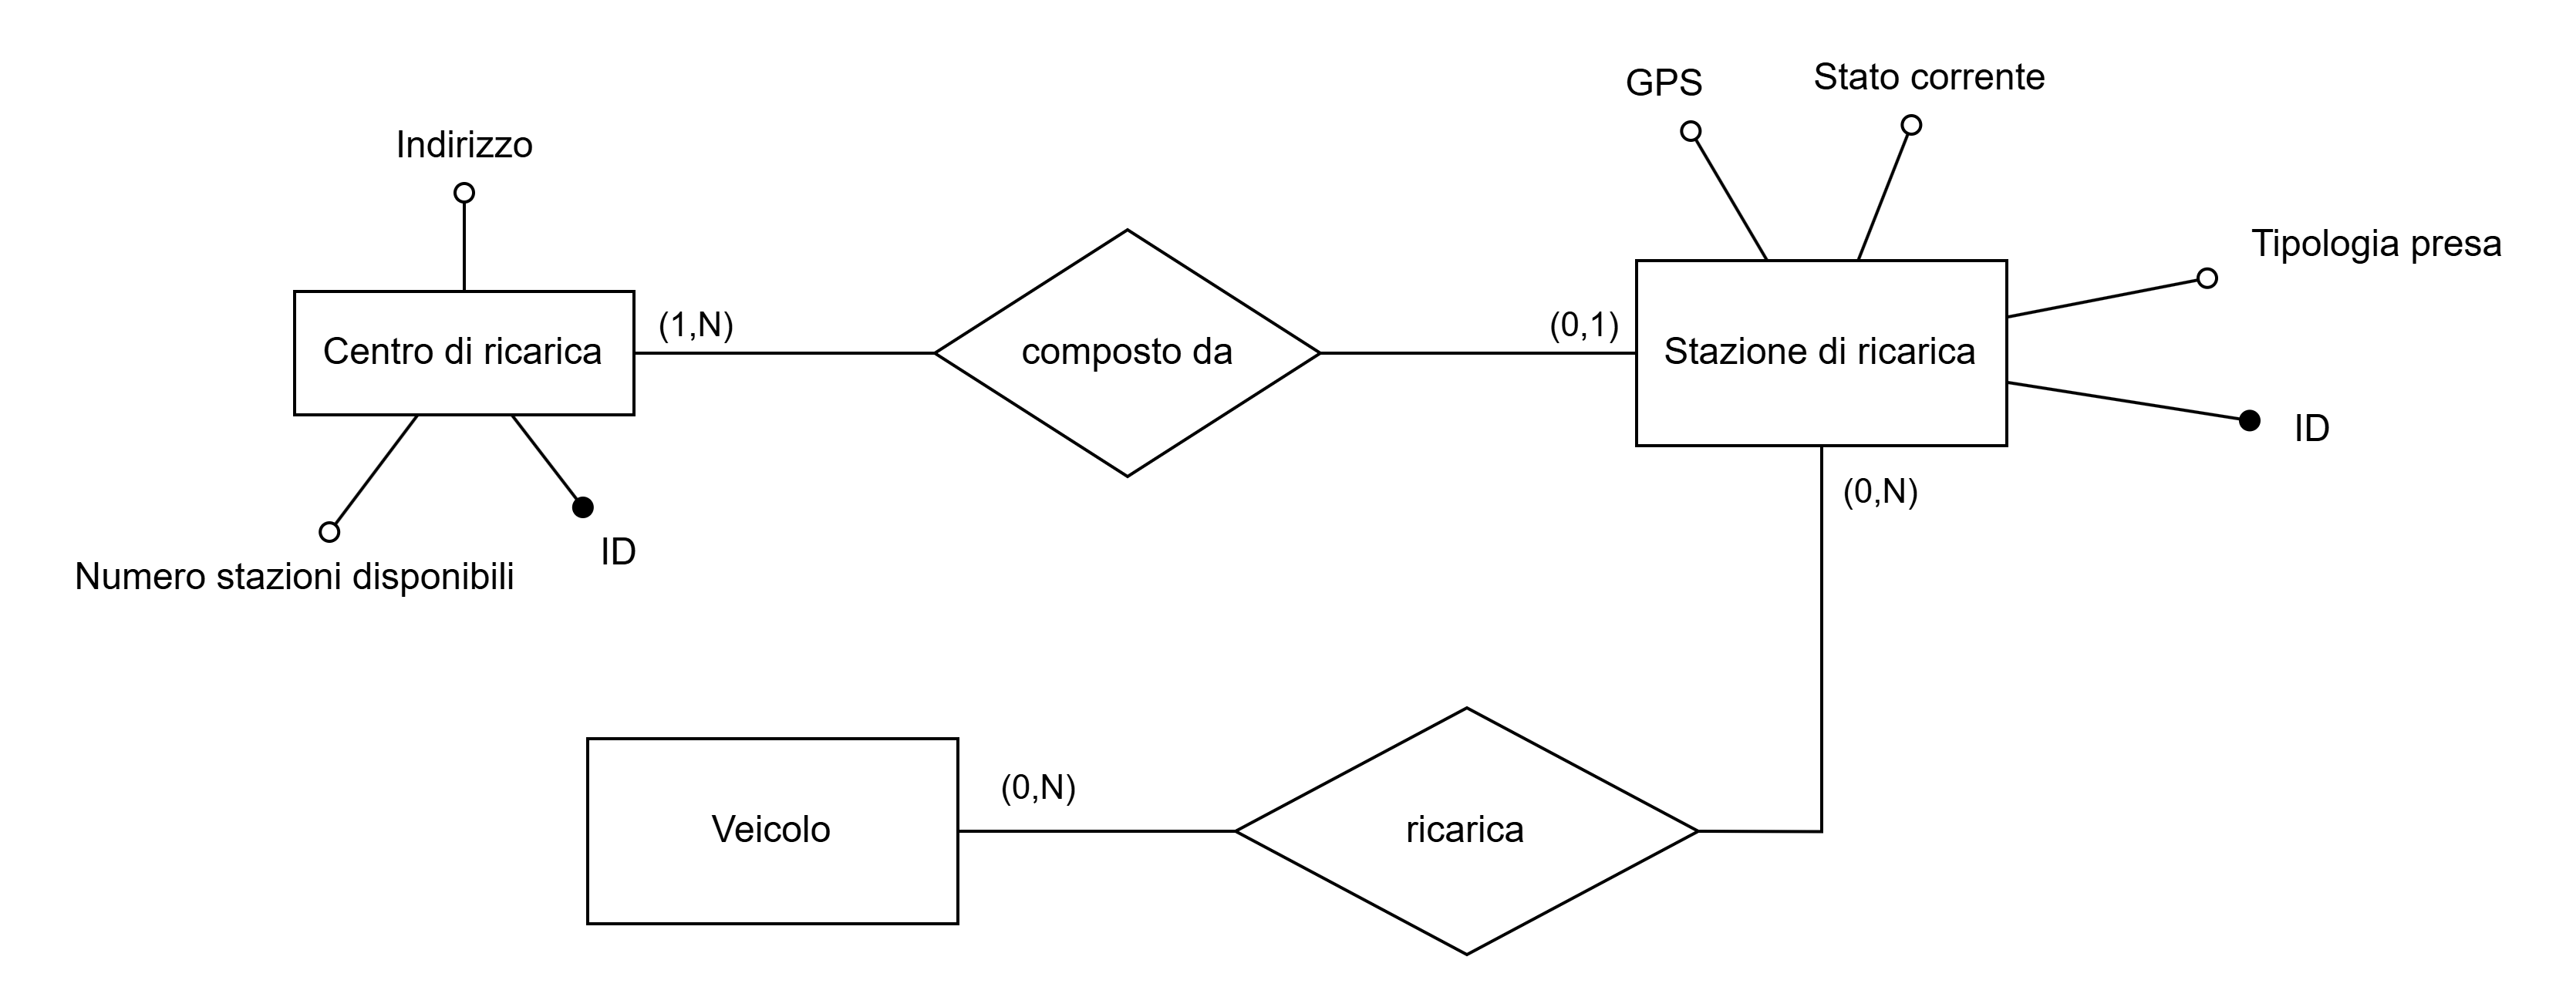
\includegraphics[width=1\linewidth]{bottom-up-ricarica.png}
    \caption{Schema E.R. della ricarica}
    \label{fig:bottom-up-ricarica}
\end{figure}

% \subsection{Unione delle componenti nello schema finale ridotto}

\clearpage

\newgeometry{margin=5pt}

\begin{figure}
    \centering
    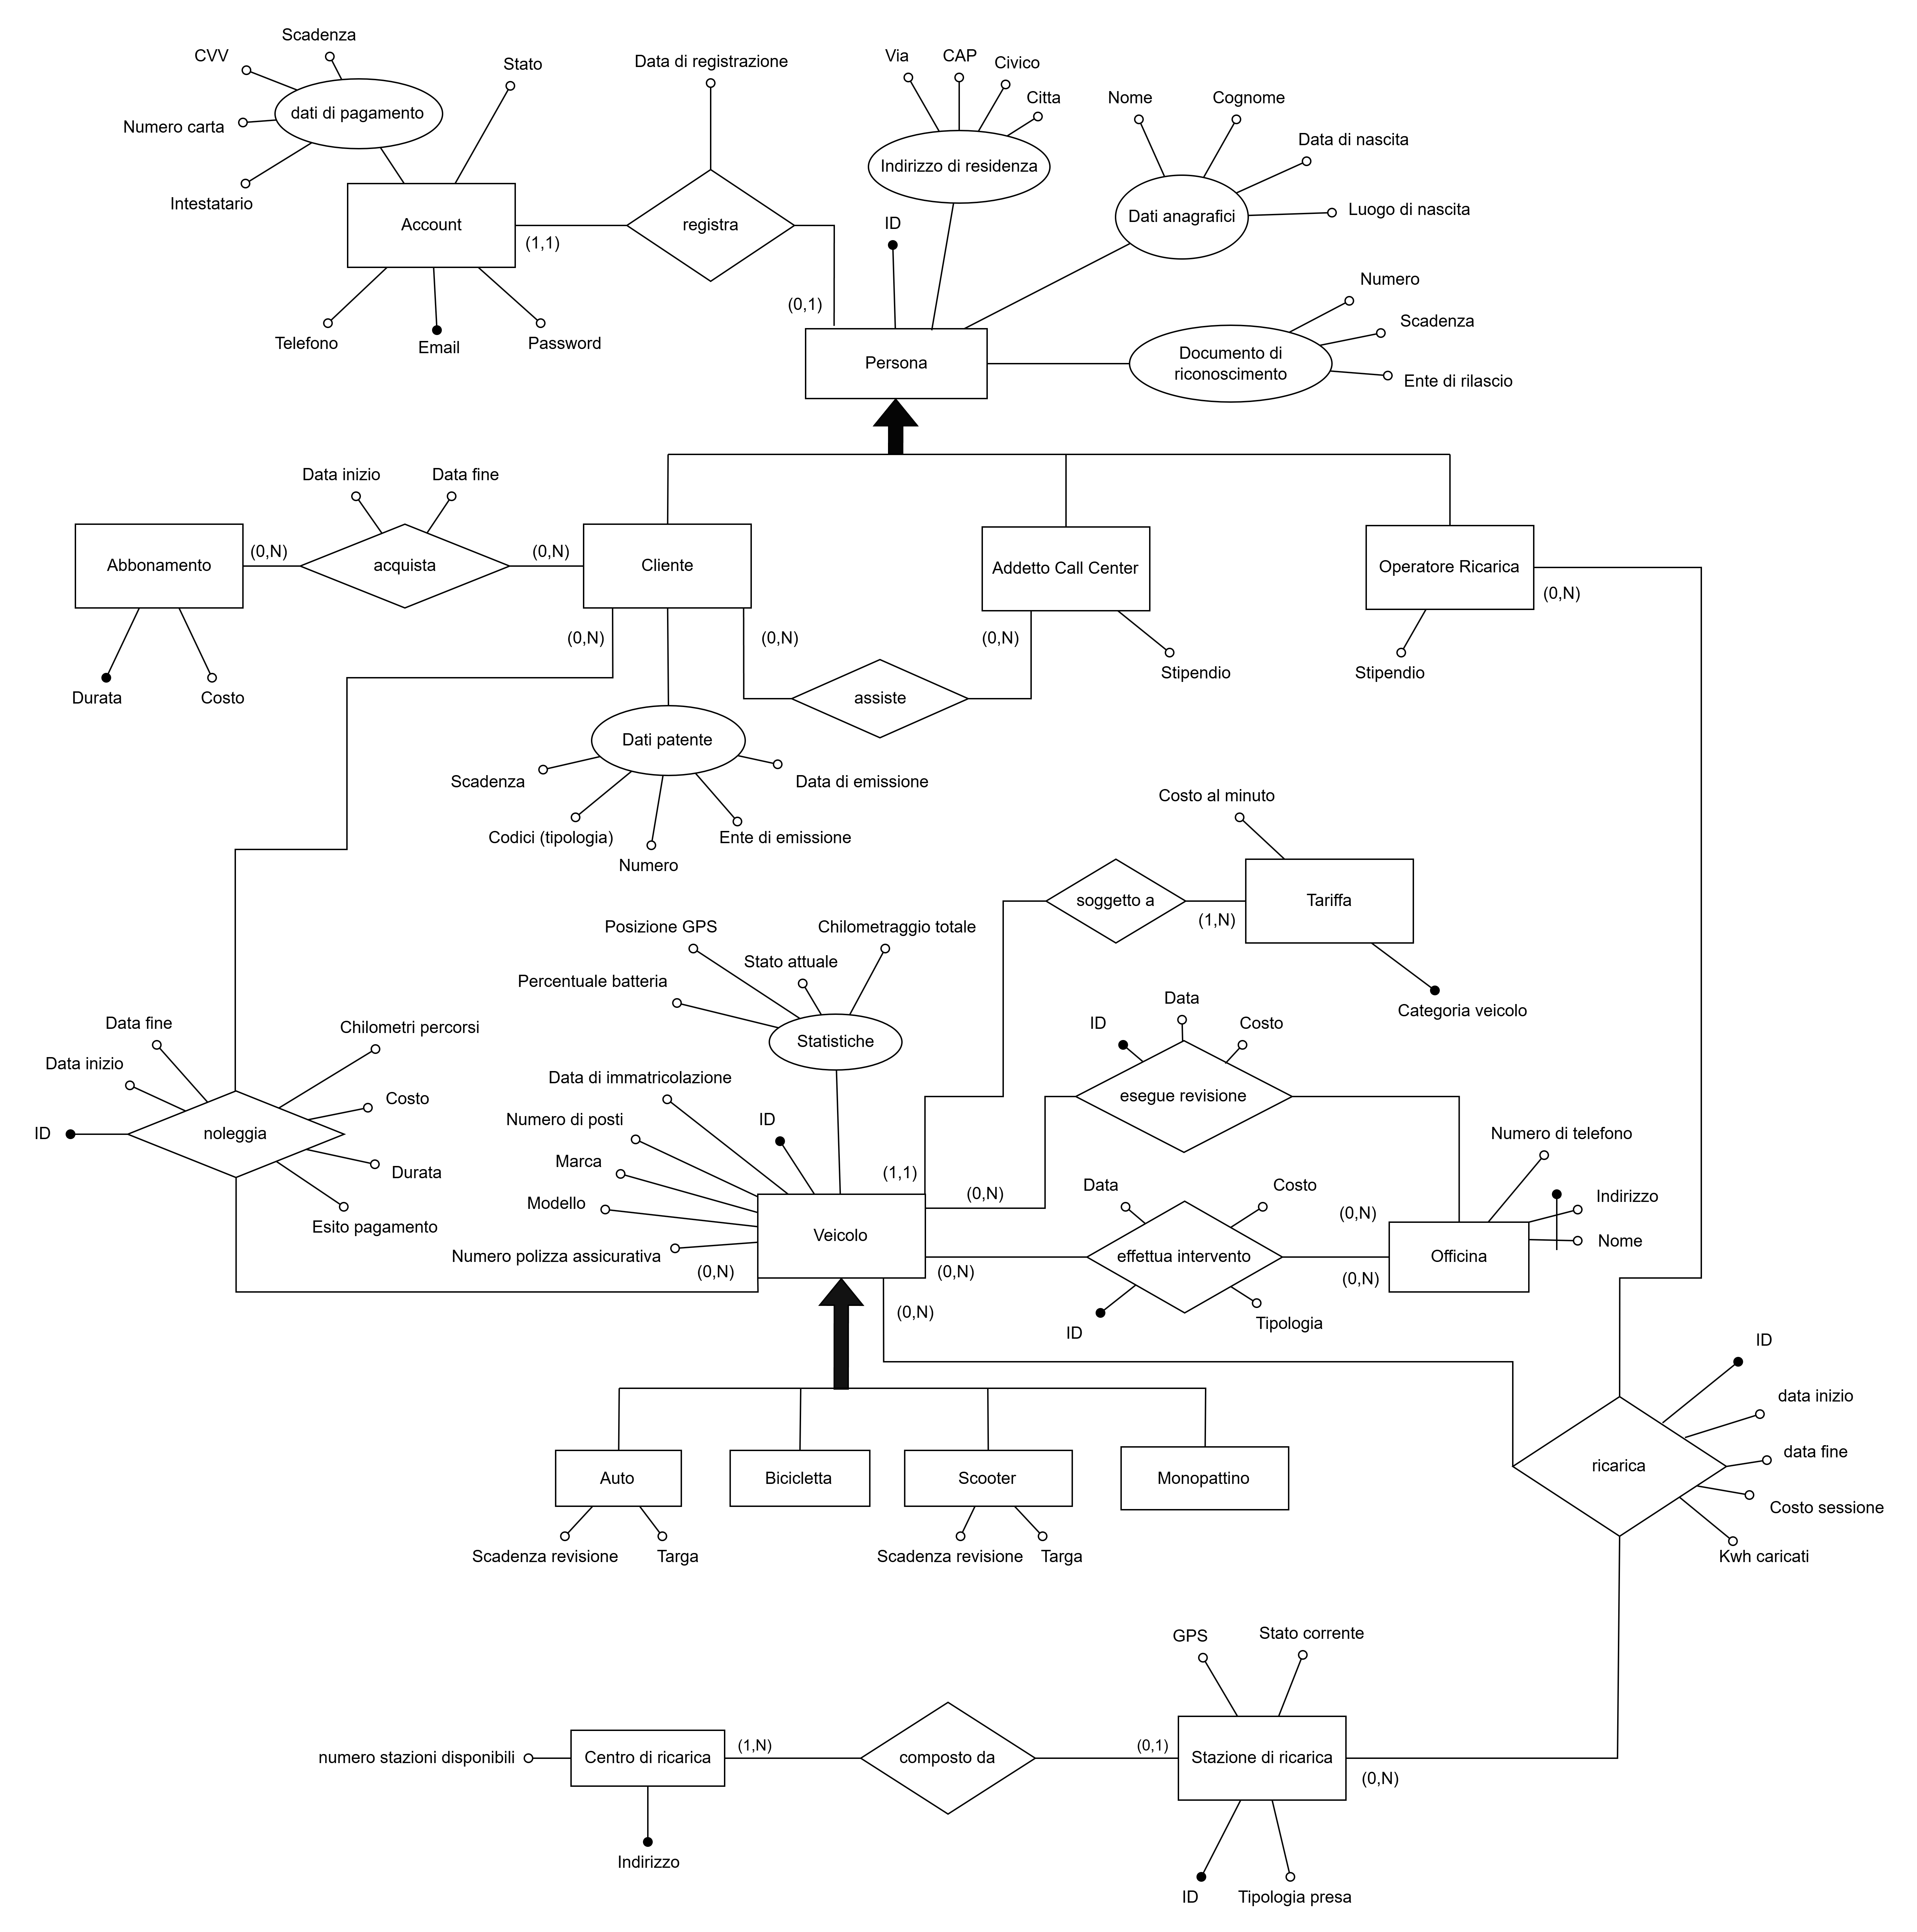
\includegraphics[
        width=0.9\paperwidth,
        height=\paperheight,
        keepaspectratio
    ]{schema-finale.png}
    \caption{Schema E.R.finale}
    \label{fig:schema-finale}
\end{figure}

\restoregeometry

\subsection{Dizionario dei dati}

\begin{longtable}[H]{|p{2.5cm}|p{4.8cm}|p{4.8cm}|p{2.3cm}|}
\hline
\textbf{Nome entità} & \textbf{Descrizione} & \textbf{Attributi} & \textbf{Identificatore} \\
\hline
\endfirsthead
\hline
\textbf{Nome entità} & \textbf{Descrizione} & \textbf{Attributi} & \textbf{Identificatore} \\
\hline
\endhead
Veicolo & Veicolo generico gestito dal servizio & Marca (stringa), Modello (stringa), Numero di posti (intero), Numero di polizza assicurativa (stringa), percentuale batteria (intero), posizione GPS (stringa), chilometraggio totale (intero), stato attuale (stringa) & ID \\ \hline
Auto & Specializzazione di veicolo & Attributi ereditati da veicolo + targa (stringa), scadenza revisione (data) & "\\ \hline
Scooter & Specializzazione di veicolo & Attributi ereditati da veicolo + targa (stringa), scadenza revisione (data) & " \\ \hline
Bicicletta & Specializzazione di veicolo & " & " \\ \hline
Monopattino & Specializzazione di veicolo & " & " \\ \hline
Persona & Generica persona & Nome (stringa), Cognome (stringa), Luogo di nascita (stringa), Data di nascita (data), Dati documento di riconoscimento (numero, data rilascio, ente rilascio, scadenza), Indirizzo di residenza (stringa) & ID \\ \hline
Account & Profilo utente associato a una persona & Email (stringa), Numero di telefono (intero), hash password (stringa), Stato (stringa), Dati di pagamento con Numero carta (intero), CVV (intero), Scadenza (data) e Intestatario (stringa) & " \\ \hline
Cliente & Utente utilizzatore del servizio di sharing & Persona + Dati patente con Numero (intero), Scadenza (data), Data di Emissione (data), Ente di Emissione (stringa), Codici (stringa) & " \\ \hline
Operatore ricarica & Persona incaricata della ricarica dei veicoli & Stipendio (intero) & " \\ \hline
Addetto call center & Persona incaricata dell'assistenza clienti telefonica per informazioni o segnalazione guasti & Stipendio (intero) & " \\ \hline
Abbonamento & Pacchetto acquistabile che permette noleggi illimitati per un determinato periodo di tempo & Durata (stringa), Costo (intero) & Durata \\ \hline
Tariffa & Costo al minuto di ogni categoria di veicoli & Prezzo al minuto (intero), Categoria veicolo (stringa) & Categoria veicolo \\ \hline
Operatore ricarica & Persona incaricata della ricarica dei veicoli & Stipendio (intero) &  \\ \hline
Officina & Luogo per interventi di riparazione e revisione di veicoli & Nome (stringa), Indirizzo (stringa), Numero di telefono (intero) & ID \\ \hline
Stazione di ricarica & Colonnina di ricarica per veicolo & Posizione GPS (stringa), Stato corrente (stringa), Tipologia presa (stringa) & ID \\ \hline
Centro di ricarica & Luogo dotato di molteplici stazioni di ricarica & Indirizzo (stringa), Numero colonnine libere (intero) & ID \\ \hline
\caption{Tabella delle entità}
\label{table_glossario_termini}
\end{longtable}

\begin{table}[H]
\centering
\begin{tabularx}{\textwidth}{|X|X|X|X|}
\hline
\textbf{Nome associazione} & \textbf{Descrizione} & \textbf{Componenti} & \textbf{Attributi} \\ \hline
Noleggio & Transazione di utilizzo di un veicolo da parte di un cliente & Veicolo (0,N), Cliente (0,N) & Data di inizio e fine (data), GPS inizio e fine (stringa), Chilometri percorsi (intero), Costo (intero), Durata (intero), Esito pagamento (stringa), ID (intero) \\ \hline
Registra & Associa un account a una persona & Account (1,1), Persona (0,1) & Data di registrazione (data)\\ \hline
Acquista & Transazione di acquisto di un abbonamento da parte di un cliente & Abbonamento (0,N), Cliente (0,N) & Data di inizio validità (data), Data di fine validità (data) \\ \hline
Assiste & Azione di richiesta di assistenza di un cliente a un addetto & Cliente (0,N), Addetto Call Center (0,N)  & ID \\ \hline
Ricarica & Associazione ternaria tra Operatore, Stazione di ricarica e Veicolo & Veicolo (0,N), Operatore (0,N), Stazione di ricarica (0,N) & Data di inizio e fine (data), Costo sessione (intero), Energia caricata (intero) \\ \hline
Composto da & Relazione madeOf: Centro di ricarica è composto da diversi stazioni di ricarica & Centro di ricarica (1,N), Stazione di ricarica (0,1) & - \\ \hline
Esegue revisione & Esecuzione evento di revisione di un veicolo presso un officina & Veicolo (0,N), Officina (0,N) & ID (intero), Data (data), Costo (intero) \\ \hline
Effettua intervento & Esecuzione intervento di riparazione di un veicolo presso un officina & Veicolo (0,N), Officina (0,N) & ID (intero), Data (data), Costo (intero), Tipologia (stringa)  \\ \hline




\end{tabularx}
\caption{Tabella delle associazioni}
\label{table_glossario_termini}
\end{table}



\subsection{Regole aziendali}
\label{sec:regole-aziendali}

\subsubsection{Regole di vincolo}
\begin{enumerate}
    \item Per registrarsi al servizio una persona deve avere un età minima di 18 anni.
    \item Un cliente deve aver inserito una patente  di guida valida di categoria appropriata per poter noleggiare veicoli di tipo "Auto" o "Scooter"
    \item Lo stato di un cliente può essere: "attivo", "bloccato", "in fase di verifica". Un cliente con stato del profilo "bloccato" o "in fase di verifica" non può effettuare nuovi noleggi.
    \item Per poter effettuare un noleggio ogni cliente deve avere un metodo di pagamento associato al proprio account.
    \item Le date di scadenza del documento di riconoscimento deve essere successiva alla data odierna per effettuare un noleggio.
    \item La percentuale della batteria di un veicolo deve essere compresa tra 0 e 100.
    \item Un veicolo può avere uno dei seguenti stati: "disponibile", "in uso", "in ricarica", "fuori servizio".
    \item Un veicolo può essere noleggiato solo se il suo stato è "disponibile" e se il suo livello di carica della batteria è superiore a 20\%.
    \item La data di inizio noleggio deve essere precedente alla data di fine noleggio.
    \item I chilometri percorsi in un noleggio devono essere maggiori o uguali a 0.
    \item La targa, per i veicoli che la prevedono (Auto, Scooter), deve essere univoca.
    \item Un cliente non può avere più di un noleggio attivo contemporaneamente e un veicolo non può essere noleggiato da più di un cliente contemporaneamente.
    \item Lo stato di una stazione di ricarica può essere: "libera", "occupata", "fuori servizio".
    \item Ogni tipologia di veicolo (Auto, Bici, Scooter, Monopattino) deve avere una tariffa base al minuto definita.
    \item Un cliente può avere solo un abbonamento attivo alla volta.
    \item I costi dei noleggi, delle sessioni di ricarica, delle manutenzioni devono essere maggiori o uguali a 0.
\end{enumerate}

\subsubsection{Regole di derivazione}
\begin{enumerate}
    \item Il costo totale del noleggio è calcolato in base alla tariffa a tempo della tipologia di veicolo e alla durata del noleggio, a meno che il cliente non abbia attivo un abbonamento.
    \item La durata di un noleggio è calcolata come differenza tra l'ora di fine e l'ora di inizio del noleggio stesso.
    \item Il numero di colonnine libere di un centro di ricarica viene calcolato in base allo stato delle stazioni di ricarica che fanno parte di quel centro
\end{enumerate}

\newpage

\section{Progettazione logica}

\subsection{Tavole dei volumi e delle operazioni}

Si ipotizza un servizio di vehicle sharing in una città italiana di medie dimensioni operativo da un anno. \footnote{Per questi dati è stato preso in considerazione l'\href{https://osservatoriosharingmobility.it/wp-content/uploads/2024/12/Rapporto-sharing-mobility-2024.pdf}{Ottavo Rapporto nazionale sulla sharing mobility} del 2024, redatto dall'Osservatorio Nazionale Sharing Mobility}

\subsubsection{Tavola dei volumi}
\begin{table}[H]
    \centering
    \begin{tabular}{|c|c|c|}
        \hline
        Concetto & Tipo & Volume \\
        \hline
        Cliente & E &  150.000 \\
        Auto & E & 200  \\
        Scooter & E & 150  \\
        Bicicletta & E & 550  \\
        Monopattino & E & 300  \\
        Addetto ricarica & E & 50  \\
        Operatore call center & E & 25 \\
        Abbonamento & E & 3 \\
        Tariffa base & E & 4 \\
        Stazione di ricarica & E & 250 \\
        Centro di ricarica & E & 15 \\
        Officina & E & 10 \\
        Account & E & 150.075 \\
        Noleggio & R & 1.500.000 \\
        Registra & R & 150.075 \\
        Acquista (abbonamento) & R & 40.000  \\
        Assiste (cliente) & R & 10.000  \\
        Ricarica & R & 200.000 \\
        Esegue revisione & R & 175 \\ 
        Effettua intervento & R & 600 \\
        Composto da & R & 250 \\
        \hline
    \end{tabular}
    \caption{Tavola dei volumi}
    \label{tab:Tavola dei volumi}
\end{table}

\subsubsection{Tavola delle operazioni}

Le operazioni che abbiamo scelto di implementare si dividono in due gruppi: operazioni "vere", che verrebbero eseguite spesso in un sistema simile, e operazioni a fini didattici, un po' più complesse ma che in un sistema vero non avrebbero molto spazio; per questo motivo le due categorie di operazioni hanno frequenza molto diversa.

\begin{table}[H]
    \centering
    \begin{tabular}{|c|c|c|}
        \hline
        Op. & Frequenza & Motivazione \\
        \hline
        1.a & 100 volte all'anno & - \\
        1.b & 1.700.000 volte all'anno & Alla fine di ogni noleggio e ricarica \\
        1.c & 50 volte all'anno & - \\
        1.d & 3.000.000 volte all'anno & - \\
        1.e & 50 volte all'anno & - \\
        1.f & 100 volte all'anno & - \\
        2.a & 1.500.000 volte all'anno & - \\
        2.b & 1.500.000 volte all'anno & Alla fine di ogni noleggio \\
        2.c & 50 volte all'anno & - \\
        2.d & 100 volte all'anno & - \\
        2.e & 12 volte all'anno & - \\
        3.a & 15.000 volte all'anno & - \\
        3.b & 30.000 volte all'anno & - \\
        3.c & 1.500 volte all'anno & - \\
        3.d & 50 volte all'anno & - \\
        3.e & 200 volte all'anno & - \\
        3.f & 20 volte all'anno & - \\
        4.a & 775 volte all'anno & 175 revisioni (ogni 2 anni per auto/scooter) + 600 interventi \\
        4.b & 12 volte all'anno & - \\
        4.c & 600 volte all'anno  & - \\
        4.d & 12 volte all'anno & - \\
        5.a & 200.000 volte all'anno & - \\
        5.b & 200.000 volte all'anno & Alla fine di ogni ricarica \\
        5.c & 12 volte all'anno &  \\
        5.d & 12 volte all'anno &  \\
        6.a & 2 volte all'anno & - \\
        6.b & 100 volte all'anno & - \\
        6.c & 1 volta all'anno & - \\
        6.d & 220.000 volte all'anno & - \\
        7.a & 30 volte all'anno & -\\
        7.b & 400.500 volte all'anno & A inizio e fine ricarica (2x200.000) + manutenzioni (500) \\
        7.c & 100 volte all'anno & - \\
        7.d & 150 volte all'anno & - \\
        8.a & 12 volte all'anno & Sconti e promozioni \\
        \hline
    \end{tabular}
    \caption{Tavola delle operazioni}
    \label{tab:Tavola delle operazioni}
\end{table}


\subsection{Ristrutturazione dello schema concettuale}

La ristrutturazione dello schema ER richiede di eliminare le ridondanze, le generalizzazioni e gli attributi composti/multivalore dato che non sono direttamente traducibili nel modello logico relazionale. 

% TODO

\subsubsection{Eliminazione delle ridondanze}
Per quanto riguarda le ridondanze, nel capitolo \ref{regole-aziendali} ne abbiamo identificate 2:

\begin{enumerate}
    \item numero di stazioni libere in un centro di ricarica, calcolabile contando le colonnine appartenenti a quel centro di ricarica che hanno stato "libera"
    \item durata del noleggio, calcolabile come differenza tra ora di fine e ora di inizio del noleggio
\end{enumerate}

Anche il costo potrebbe sembrare una ridondanza (calcolato come durata*tariffa al minuto), ma in realtà dato che le tariffe al minuto possono variare nel corso del tempo è necessario salvarsi il costo al momento del salvataggio del noleggio.

Per decidere se mantenere o rimuovere le ridondanze, analizziamo il costo delle varie operazioni considerando doppio il costo di una scrittura rispetto a una lettura.

La prima ridondanza riguarda l'attributo "numero di stazioni di ricarica libere" in centro di ricarica
derivabili dal conteggio delle stazioni di ricarica con attributo "stato corrente" = libera.
Influenza le operazioni 7.b (modifica stato stazione di ricarica) e 6.d (visualizzazione dei centri di ricarica ordinati per numero di colonnine libere).

\begin{table}[h]
  \centering
  \begin{tabular}{|c|c|c|c|}
    \hline
    Tabella & Costrutto & Accessi & Tipo op \\ \hline
    Centro di ricarica  & E & 1 & R \\ \hline
  \end{tabular}
  \caption{Tavola accessi op. 6.d in presenza di ridondanza}
  \label{tab:label}
\end{table}

\begin{table}[h]
  \centering
  \begin{tabular}{|c|c|c|c|}
    \hline
    Tabella & Costrutto & Accessi & Tipo op \\ \hline
    Centro di ricarica  & E & 1 & R \\ \hline
    Stazione di ricarica & E & 17 & R \\ \hline
  \end{tabular}
  \caption{Tavola accessi op. 6.d in assenza di ridondanza}
  \label{tab:label}
\end{table}

\begin{table}[h]
  \centering
  \begin{tabular}{|c|c|c|c|}
    \hline
    Tabella & Costrutto & Accessi & Tipo op \\ \hline
    Stazione di ricarica  & E & 1 & W \\ \hline 
    Stazione di ricarica  & E & 1 & R \\ \hline % perchè devo leggere l'ID del centro di ricarica associato alla stazione di ricarica
    Centro di ricarica  & E & 1 & R \\ \hline % perchè devo leggere il valore del counter attuale
    Centro di ricarica  & E & 1 & W \\ \hline % perchè devo incrementare il valore del counter 
  \end{tabular}
  \caption{Tavola accessi op. 7.b in presenza di ridondanza}
  \label{tab:label}
\end{table}

\begin{table}[h]
  \centering
  \begin{tabular}{|c|c|c|c|}
    \hline
    Tabella & Costrutto & Accessi & Tipo op \\ \hline
    Stazione di ricarica & E & 1 & W \\ \hline
  \end{tabular}
  \caption{Tavola accessi op. 7.b in assenza di ridondanza}
  \label{tab:label}
\end{table}

In presenza di ridondanza: 

\begin{itemize}
    \item Operazione 7.b effettuata 400.500 volte all'anno: 6 (costo) * 400.500 = 2.403.000
    \item Operazione 6.d effettuata 220.000 volte all'anno: 1 (costo) * 220.000 = 220.000
\end{itemize}

Costo totale annuo con ridondanza: 2.403.000 + 220.000 = 2.623.000

In assenza di ridondanza: 
\begin{itemize}
    \item Operazione 7.b effettuata 400.500 volte/anno.: 2 (costo) * 400.500 = 801.000
    \item Operazione 6.d effettuata 220.000 volte/anno: 18 (costo medio) * 220.000 = 3.960.000
\end{itemize}

Costo totale annuo senza ridondanza: 801.000 + 3.960.000 = 4.761.000

Il costo totale con ridondanza è nettamente inferiore al costo senza ridondanza, quindi ci conviene tenere l'attributo ridondante.

La seconda ridondanza riguarda l'attributo "durata" di noleggio che può essere calcolato utilizzando gli attributi "data inizio" e "data fine". 

Le operazioni influenzate da queste ridondanza sono: 2.b (aggiornamento dei dati alla conclusione del noleggio) e 2.c (visualizzazione della durata media dei noleggi). 

\begin{table}[h]
  \centering
  \begin{tabular}{|c|c|c|c|}
    \hline
    Tabella & Costrutto & Accessi & Tipo op \\ \hline
    Noleggio & R & 1 & R  \\ \hline % Per leggere data di inizio? 
    Noleggio & R & 1 & W  \\ \hline 
  \end{tabular}
  \caption{Tavola accessi op. 2.b in presenza di ridondanza}
\end{table}

\begin{table}[h]
  \centering
  \begin{tabular}{|c|c|c|c|}
    \hline
    Tabella & Costrutto & Accessi & Tipo op \\ \hline
    Noleggio & R & 1 & W \\ \hline 
  \end{tabular}
  \caption{Tavola accessi op. 2.b in assenza di ridondanza}
\end{table}

\begin{table}[h]
  \centering
  \begin{tabular}{|c|c|c|c|}
    \hline
    Tabella & Costrutto & Accessi & Tipo op \\ \hline
    Veicolo & E & 1.200 & R  \\ \hline
    Noleggio & R & 1.500.000 & R \\ \hline
  \end{tabular}
  \caption{Tavola accessi op. 2.c in presenza di ridondanza}
\end{table}

\begin{table}[h]
  \centering
  \begin{tabular}{|c|c|c|c|}
    \hline
    Tabella & Costrutto & Accessi & Tipo op \\ \hline
    Veicolo & E & 1.200 & R  \\ \hline
    Noleggio & R & 1.500.000 & R \\ \hline
  \end{tabular}
  \caption{Tavola accessi op. 2.c in assenza di ridondanza}
\end{table}

Dato che l'operazione 2.c non cambia il costo in presenza o assenza di ridondanza possiamo calcolare il costo annuo solo dell'operazione 2.b.
Costo attuale con ridondanza: 3 (costo) * 1.500.000 = 4.500.000
Costo annuale senza ridondanza: 2 (costo) * 1.500.000 = 3.000.000

Il costo totale annuo in assenza di ridondanza è inferiore, quindi abbiamo deciso di rimuovere l'attributo "Durata".


I seguenti attributi composti vengono scomposti e inseriti come attributi dell'entità.
\begin{itemize}
    \item dati anagrafici: comprendono nome, cognome, data di nascita e luogo di nascita
    \item statistiche veicolo: comprendono percentuale batteria, posizione GPS, chilometraggio totale e stato attuale.
    \item gli attributi via, civico, CAP e città di indirizzo di residenza vengono inseriti in unico attributo Indirizzo (stringa)
\end{itemize}


\subsubsection{Eliminazione delle gerarchie}

Riguardo la generalizzazione Persona abbiamo deciso di rimuovere l'entità padre Persona e mantenere le 3 diverse entità figlie: Cliente, Addetto alla ricarica e Operatore Call Center; seppur presentano attributi comuni, hanno relazioni diverse all'interno del servizio e pertanto è necessario mantenerle separate.

Per i veicoli abbiamo deciso di fare parent embedding: quindi mantenere solamente l'entità Veicolo aggiungendo l'attributo tipologia e inserendo due attributi opzionali (targa, scadenza revisione) 

\subsubsection{Accorpamenti e partizioni}
L'attributo composto \textsc{dati patente} viene partizionato in un entità \textsc{Patente} con attributi Numero (chiave primaria), dati di emissione, ente di emissione, scadenza, codici; l'entità Cliente sarà in relazione (0,1) con Patente.
L'attributo composto \textsc{dati di pagamento} viene partizionato in un'entità Metodo di Pagamento con attributi numero carta (chiave primaria), intestatario, scadenza, CVV; l'entità Cliente sarà in relazione (0,N) con Metodo di Pagamento.
Allo stesso modo, l'attributo composto \textsc{documento di riconoscimento} viene partizionato in una nuova entità \textsc{Carta d'Identità}; Cliente sarà allora in relazione (0,1) con Carta d'Identità.
L'attributo composto \textsc{documento di riconoscimento} viene partizionato in una nuova entità Documento con attributi Numero, Scadenza, Ente rilascio.

\subsubsection{Eliminazione degli attributi multivalore}
Non abbiamo riscontrato la presenza di attributi multivalore nella nostra base di dati.


\subsubsection{Elenco degli identificatori principali}

\begin{table}[H]
    \centering
    \begin{tabular}{|c|c|}
    \hline
        \textbf{Nome entità} & \textbf{Identificatore} \\ \hline
        Account & ID \\
        Cliente & ID \\
        Addetto Call Center & ID \\
        Operatore Ricarica & ID \\
        Abbonamento & Durata \\
        Documento di riconoscimento & Numero \\
        Patente & Numero \\
        Metodo di pagamento & ID \\
        Veicolo & ID \\
        Tariffa & Categoria veicolo \\
        Officina & ID \\
        Stazione di ricarica & ID \\
        Centro di ricarica & ID \\ 
        \hline
    \end{tabular}
    \caption{Identificatori principali}
    \label{tab:identificatori-principali}
\end{table}

\subsection{Normalizzazione}

\subsubsection{Associazioni}

Dopo la ristrutturazione dello schema concettuale, tutte le associazioni presenti nello schema aggiornato non presentano anomalie e sono in forma normale di Boyce Codd. 

\subsubsection{Entità}

Anche per quanto riguarda le entità, dopo i dovuti partizionamenti decisi durante la ristrutturazione dello schema, risulta che nessuna di esse presenta dipendente non banali tra attributi e pertanto sono tutte in forma normale.

\subsection{Traduzione verso il modello relazionale}

\subsubsection{Entità-relazione}


\begin{table}[H]
    \centering
    \begin{tabularx}{\textwidth}{|p{3.1cm}|X|}
    \hline
        \textbf{Entità - Relazione} & \textbf{Traduzione} \\ \hline
        Account & Account(\underline{ID}, Email, Password, Telefono, Stato, Dipendente, MetodoPagamento, DataRegistrazione) \\ \hline
        Cliente & Cliente(\underline{AccountID}, Nome, Cognome, DataNascita, LuogoNascita, Indirizzo, Patente, Documento)\\ \hline
        Addetto Call Center & AddettoCallCenter(\underline{AccountID}, Nome, Cognome, DataNascita, Indirizzo, Stipendio)\\ \hline 
        Operatore Ricarica & OperatoreRicarica(\underline{AccountID}, Nome, Cognome, DataNascita, LuogoNascita, Indirizzo, Stipendio)\\ \hline
        Abbonamento & Abbonamento(\underline{Durata}, Costo)\\ \hline
        Documento & Documento(\underline{Numero}, Scadenza, EnteRilascio)\\ \hline
        Patente & Patente(\underline{Numero}, Scadenza, EnteRilascio, DataRilascio, AutoAbilitata)  \\ \hline
        MetodoPagamento & MetodoPagamento(\underline{ID}, NumeroCarta, Intestatario, CVV, Scadenza) \\ \hline
        Veicolo & Veicolo(\underline{ID}, Targa, Tipologia, ScadenzaRevisione, PolizzaAssicurazione, Modello, Marca, NumeroPosti, DataImmatricolazione, PercentualeBatteria, GPS, Stato, ChilometraggioTotale)\\ \hline
        Tariffa & Tariffa(\underline{CategoriaVeicolo}, CostoAlMinuto)\\ \hline
        Officina & Officina(\underline{ID}, Nome, Indirizzo, NumeroTelefono) \\ \hline
        StazioneRicarica & StazioneRicarica(\underline{ID}, TipologiaPresa, GPS, Stato, CentroRicarica) \\ \hline
        CentroRicarica & CentroRicarica(\underline{ID}, Indirizzo, StazioniDisponibili) \\ \hline
        Noleggia & Noleggia(\underline{ID}, Cliente, VeicoloID, DataInizio, DataFine, ChilometriPercorsi, GPSInizio, GPSFine, Costo, EsitoPagamento)\\ \hline
        Assiste & Assiste(\underline{ID}, AddettoAccountID, Cliente, DataRichiesta, ProblemaRiscontrato, Stato)\\ \hline
        Acquista & Acquisti\_Abbonamenti(\underline{ID}, Cliente, TipoAbbonamento, DataInizioValidita, DataFineValidita) \\ \hline
        Esegue Revisione & EsegueRevisione(\underline{ID}, VeicoloID, OfficinaID, Data, Costo, Note) \\ \hline
        Esegue Intervento & EsegueIntervento(\underline{ID}, VeicoloID, OfficinaID, Data, Costo, Tipologia, Descrizione)\\ \hline
        Ricarica & Ricarica(\underline{ID}, Operatore, VeicoloID, StazioneRicarica, DataInizio, DataFine, CostoSessione, KWhCaricati) \\ \hline
    \end{tabularx}
    \caption{Verso il modello relazionale: entità-relazioni}
    \label{tab:entità-relazioni}
\end{table}


\subsubsection{Traduzione e vincoli di riferimento}

\begin{table}[H]
    \centering
    \begin{tabularx}{\textwidth}{|X|X|}
        \hline
        \textbf{Traduzione} & \textbf{Vincoli di riferimento} \\ \hline
        Account(\underline{ID}, Email, Password, Telefono, Stato, Dipendente, MetodoPagamento, DataRegistrazione) & MetodoPagamento \(\to\) MetodoPagamento.ID \\ \hline
        Cliente(\underline{AccountID}, Nome, Cognome, DataNascita, LuogoNascita, Indirizzo, Patente, Documento) & AccountID \(\to\) Account.ID, Patente \(\to\) Patente.Numero, Documento \(\to\) Documento.Numero \\ \hline
        AddettoCallCenter(\underline{AccountID}, Nome, Cognome, DataNascita, Indirizzo, Stipendio) & AccountID \(\to\) Account.ID \\ \hline
        OperatoreRicarica(\underline{AccountID}, Nome, Cognome, DataNascita, LuogoNascita, Indirizzo, Stipendio) & AccountID \(\to\) Account.ID \\ \hline
        Abbonamento(\underline{Durata}, Costo) & \\ \hline
        Documento(\underline{Numero}, Scadenza, EnteRilascio) & \\ \hline
        Patente(\underline{Numero}, Scadenza, EnteRilascio, DataRilascio, AutoAbilitata) & \\ \hline
        MetodoPagamento(\underline{ID}, NumeroCarta, Intestatario, CVV, Scadenza) & \\ \hline
        Veicolo(\underline{ID}, Targa, Tipologia, ScadenzaRevisione, PolizzaAssicurazione, Modello, Marca, NumeroPosti, DataImmatricolazione, PercentualeBatteria, GPS, Stato, ChilometraggioTotale) & Tipologia \(\to\) Tariffa.CategoriaVeicolo \\ \hline
        Tariffa(\underline{CategoriaVeicolo}, CostoAlMinuto) & \\ \hline
        Officina(\underline{ID}, Nome, Indirizzo, NumeroTelefono) & \\ \hline
        StazioneRicarica(\underline{ID}, TipologiaPresa, GPS, Stato, CentroRicarica) & CentroRicarica \(\to\) CentroRicarica.ID \\ \hline
        CentroRicarica(\underline{ID}, Indirizzo, StazioniDisponibili) & \\ \hline
        Noleggia(\underline{ID}, Cliente, VeicoloID, DataInizio, DataFine, ChilometriPercorsi, GPSInizio, GPSFine, Costo, EsitoPagamento) & Cliente \(\to\) Cliente.AccountID, VeicoloID \(\to\) Veicolo.ID \\ \hline
        Assiste(\underline{ID}, AddettoAccountID, Cliente, DataRichiesta, ProblemaRiscontrato, Stato) & AddettoAccountID \(\to\) AddettoCallCenter.AccountID, Cliente \(\to\) Cliente.AccountID \\ \hline
        Acquisti\_Abbonamenti(\underline{ID}, Cliente, TipoAbbonamento, DataInizioValidita, DataFineValidita) & Cliente \(\to\) Cliente.AccountID, TipoAbbonamento \(\to\) Abbonamento.Durata \\ \hline
        EsegueRevisione(\underline{ID}, VeicoloID, OfficinaID, Data, Costo, Note) & VeicoloID \(\to\) Veicolo.ID, OfficinaID \(\to\) Officina.ID \\ \hline
        EsegueIntervento(\underline{ID}, VeicoloID, OfficinaID, Data, Costo, Tipologia, Descrizione) & VeicoloID \(\to\) Veicolo.ID, OfficinaID \(\to\) Officina.ID \\ \hline
        Ricarica(\underline{ID}, Operatore, VeicoloID, StazioneRicarica, DataInizio, DataFine, CostoSessione, KWhCaricati) & Operatore \(\to\) OperatoreRicarica.AccountID, VeicoloID \(\to\) Veicolo.ID, StazioneRicarica \(\to\) StazioneRicarica.ID \\ \hline
    \end{tabularx}
    \caption{Verso il modello relazionale: entità-relazioni (traduzioni uniformate)}
    \label{tab:entita-relazioni-tradotte}
\end{table}



\newgeometry{margin=5pt}

\begin{figure}
    \centering
    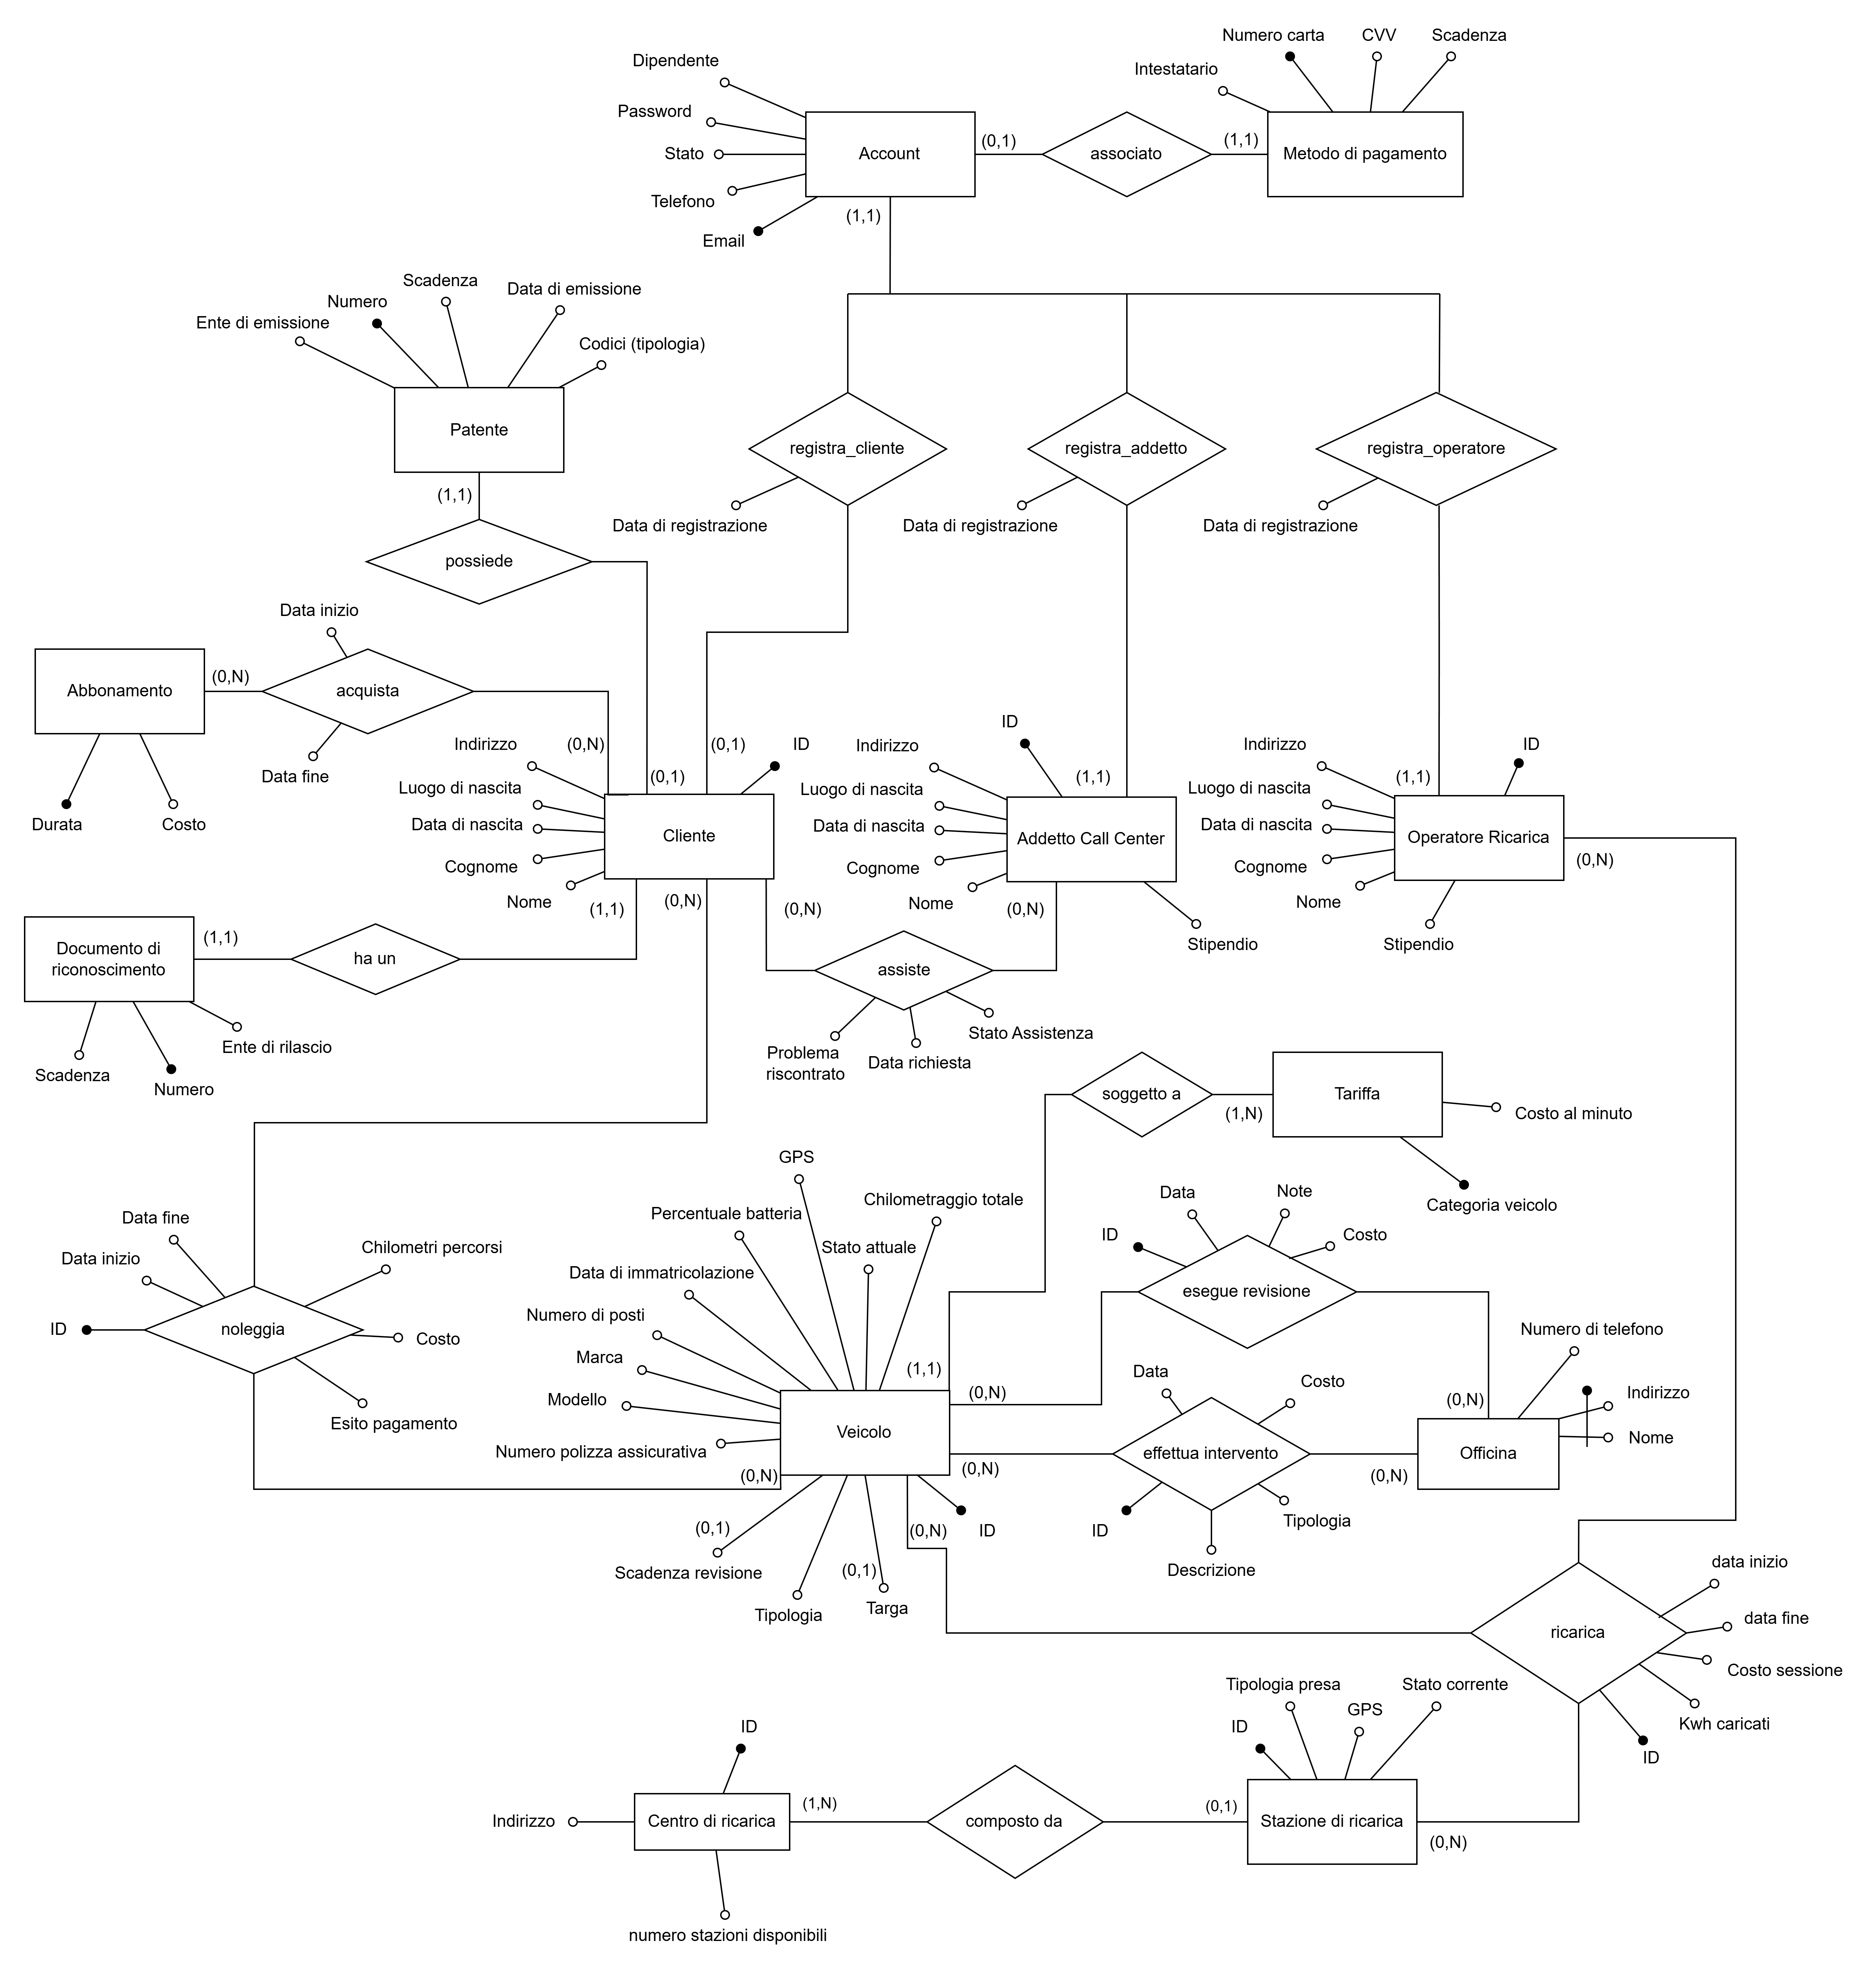
\includegraphics[
        width=0.9\paperwidth,
        height=\paperheight,
        keepaspectratio
    ]{schema-ristrutturato.png}
    \caption{Schema E.R. ristrutturato}
    \label{fig:schema-ristrutturato}
\end{figure}

\restoregeometry


\section{Codifica SQL}

\subsection{Definizione dello schema}

\begin{lstlisting}
CREATE TABLE MetodoPagamento (
    ID INT AUTO_INCREMENT PRIMARY KEY,
    NumeroCarta VARCHAR(25) NOT NULL UNIQUE,
    Intestatario VARCHAR(255) NOT NULL,
    CVV VARCHAR(4) NOT NULL, 
    Scadenza DATE NOT NULL, 
    CONSTRAINT check_carta CHECK 
    (
        LENGTH(NumeroCarta) BETWEEN 13 AND 19 AND 
        NumeroCarta REGEXP '^[0-9]+$'
    )
);

CREATE TABLE Account (
    ID INT AUTO_INCREMENT PRIMARY KEY,
    Email VARCHAR(255) NOT NULL UNIQUE,
    Password VARCHAR(255) NOT NULL, 
    Telefono VARCHAR(20) UNIQUE,
    Stato ENUM('attivo', 'bloccato', 'in_fase_di_verifica', 'eliminato') NOT NULL DEFAULT 'in_fase_di_verifica',
    Dipendente BOOLEAN NOT NULL DEFAULT FALSE, 
    MetodoPagamento VARCHAR(25) NULL,
    DataRegistrazione DATETIME NOT NULL DEFAULT CURRENT_TIMESTAMP,
    FOREIGN KEY (MetodoPagamento) REFERENCES MetodoPagamento(NumeroCarta) ON DELETE SET NULL ON UPDATE CASCADE
);

CREATE TABLE Documento (
    Numero VARCHAR(50) PRIMARY KEY,
    Scadenza DATE NOT NULL,
    EnteRilascio VARCHAR(100) NOT NULL
);

CREATE TABLE Patente (
    Numero VARCHAR(50) PRIMARY KEY,
    Scadenza DATE NOT NULL,
    EnteRilascio VARCHAR(100) NOT NULL,
    DataRilascio DATE NOT NULL,
    AutoAbilitata BOOLEAN NOT NULL 
);

CREATE TABLE Tariffa (
    CategoriaVeicolo ENUM('auto', 'scooter', 'bicicletta', 'monopattino') PRIMARY KEY,
    CostoAlMinuto DECIMAL(3, 2) NOT NULL CHECK (CostoAlMinuto >= 0)
);

CREATE TABLE Officina (
    ID INT AUTO_INCREMENT PRIMARY KEY,
    Nome VARCHAR(255) NOT NULL,
    Indirizzo VARCHAR(255) NOT NULL,
    NumeroTelefono VARCHAR(20)
);

CREATE TABLE Abbonamento (
    Durata ENUM('giornaliero', 'settimanale', 'mensile') PRIMARY KEY, 
    Costo DECIMAL(5, 2) NOT NULL CHECK (Costo >= 0)
);

CREATE TABLE CentroRicarica (
    ID INT AUTO_INCREMENT PRIMARY KEY,
    Indirizzo VARCHAR(255) NOT NULL UNIQUE,
    StazioniDisponibili INT NOT NULL DEFAULT 0 CHECK (StazioniDisponibili >= 0)
);

CREATE TABLE Cliente (
    AccountID INT PRIMARY KEY,
    Nome VARCHAR(100) NOT NULL,
    Cognome VARCHAR(100) NOT NULL,
    DataNascita DATE NOT NULL, 
    LuogoNascita VARCHAR(100) NOT NULL,
    Indirizzo VARCHAR(255) NOT NULL, 
    Patente VARCHAR(50) NULL, 
    Documento VARCHAR(50) NOT NULL, 
    FOREIGN KEY (AccountID) REFERENCES Account(ID) ON DELETE RESTRICT ON UPDATE CASCADE,
    FOREIGN KEY (Patente) REFERENCES Patente(Numero) ON DELETE RESTRICT ON UPDATE CASCADE,
    FOREIGN KEY (Documento) REFERENCES Documento(Numero) ON DELETE RESTRICT ON UPDATE CASCADE
);

CREATE TABLE AddettoCallCenter (
    AccountID INT PRIMARY KEY,
    Nome VARCHAR(100) NOT NULL,
    Cognome VARCHAR(100) NOT NULL,
    DataNascita DATE NOT NULL,
    LuogoNascita VARCHAR(100),
    Indirizzo VARCHAR(255),
    Stipendio DECIMAL(7, 2),
    FOREIGN KEY (AccountID) REFERENCES Account(ID) ON DELETE CASCADE ON UPDATE CASCADE
);

CREATE TABLE OperatoreRicarica (
    AccountID INT PRIMARY KEY,
    Nome VARCHAR(100) NOT NULL,
    Cognome VARCHAR(100) NOT NULL,
    DataNascita DATE NOT NULL,
    LuogoNascita VARCHAR(100),
    Indirizzo VARCHAR(255),
    Stipendio DECIMAL(7, 2),
    FOREIGN KEY (AccountID) REFERENCES Account(ID) ON DELETE CASCADE ON UPDATE CASCADE
);

CREATE TABLE Veicolo (
    ID INT AUTO_INCREMENT PRIMARY KEY,
    Targa VARCHAR(10) NULL UNIQUE, 
    ScadenzaRevisione DATE NULL, 
    PolizzaAssicurazione VARCHAR(100) NOT NULL,
    Modello VARCHAR(100) NOT NULL,
    Marca VARCHAR(100) NOT NULL,
    NumeroPosti INT DEFAULT 1 CHECK (NumeroPosti >= 1),
    DataImmatricolazione DATE NULL,
    PercentualeBatteria INT NOT NULL DEFAULT 100 CHECK (PercentualeBatteria BETWEEN 0 AND 100),
    GPS POINT NOT NULL, 
    Stato ENUM('disponibile', 'in_uso', 'in_ricarica', 'fuori_servizio', 'eliminato') NOT NULL DEFAULT 'disponibile',
    ChilometraggioTotale INT NOT NULL DEFAULT 0 CHECK (ChilometraggioTotale >= 0),
    Tipologia ENUM('auto', 'scooter', 'bicicletta', 'monopattino') NOT NULL,
    FOREIGN KEY (Tipologia) REFERENCES Tariffa(CategoriaVeicolo) ON DELETE RESTRICT ON UPDATE RESTRICT,
    CONSTRAINT CHK_tipo CHECK 
    (
        Tipologia = 'monopattino' OR 
        Tipologia = 'bicicletta' OR 
        (
            Tipologia IN ('auto', 'scooter') AND
            Targa IS NOT NULL AND 
            ScadenzaRevisione IS NOT NULL AND
            DataImmatricolazione IS NOT NULL
        )
    )
);

CREATE TABLE StazioneRicarica (
    ID INT AUTO_INCREMENT PRIMARY KEY,
    TipologiaPresa ENUM('Type2', 'CCS2', 'Schuko') NOT NULL,
    GPS POINT NOT NULL, 
    Stato ENUM('libera', 'occupata', 'in_manutenzione', 'fuori_servizio', 'eliminata') NOT NULL DEFAULT 'libera',
    CentroRicarica INT NULL,
    FOREIGN KEY (CentroRicarica) REFERENCES CentroRicarica(ID) ON DELETE SET NULL ON UPDATE CASCADE
);

CREATE TABLE Noleggia (
    ID INT AUTO_INCREMENT PRIMARY KEY,
    Cliente INT NOT NULL,
    VeicoloID INT NOT NULL,
    DataInizio DATETIME NOT NULL DEFAULT CURRENT_TIMESTAMP,
    DataFine DATETIME NULL,
    GPSInizio POINT NULL, 
    GPSFine POINT NULL,
    ChilometriPercorsi INT NULL CHECK (ChilometriPercorsi IS NULL OR ChilometriPercorsi >= 0),
    Costo DECIMAL(7, 2) NULL CHECK (Costo IS NULL OR Costo >= 0),
    EsitoPagamento ENUM('successo', 'fallito', 'in_attesa') DEFAULT 'in_attesa',
    FOREIGN KEY (Cliente) REFERENCES Cliente(AccountID) ON DELETE RESTRICT ON UPDATE CASCADE,
    FOREIGN KEY (VeicoloID) REFERENCES Veicolo(ID) ON DELETE RESTRICT ON UPDATE CASCADE
);

CREATE TABLE Assiste (
    ID INT AUTO_INCREMENT PRIMARY KEY,
    AddettoAccountID INT NOT NULL,
    Cliente INT NOT NULL,
    DataRichiesta DATETIME NOT NULL DEFAULT CURRENT_TIMESTAMP,
    ProblemaRiscontrato TEXT,
    Stato ENUM('aperta', 'in_lavorazione', 'chiusa') DEFAULT 'aperta',
    FOREIGN KEY (AddettoAccountID) REFERENCES AddettoCallCenter(AccountID) ON DELETE RESTRICT ON UPDATE CASCADE,
    FOREIGN KEY (Cliente) REFERENCES Cliente(AccountID) ON DELETE RESTRICT ON UPDATE CASCADE
);

CREATE TABLE Acquisti_Abbonamenti (
    ID INT AUTO_INCREMENT PRIMARY KEY,
    Cliente INT NOT NULL,
    TipoAbbonamento ENUM('giornaliero', 'settimanale', 'mensile') NOT NULL,
    DataInizioValidita DATE NOT NULL,
    DataFineValidita DATE NOT NULL,
    FOREIGN KEY (Cliente) REFERENCES Cliente(AccountID) ON DELETE RESTRICT ON UPDATE CASCADE,
    FOREIGN KEY (TipoAbbonamento) REFERENCES Abbonamento(Durata) ON DELETE RESTRICT ON UPDATE RESTRICT
);

CREATE TABLE EsegueRevisione (
    ID INT AUTO_INCREMENT PRIMARY KEY,
    VeicoloID INT NOT NULL,
    OfficinaID INT NOT NULL,
    Data DATETIME NOT NULL,
    Costo DECIMAL(6, 2) NOT NULL CHECK (Costo >= 0),
    Note TEXT NULL,
    FOREIGN KEY (VeicoloID) REFERENCES Veicolo(ID) ON DELETE RESTRICT ON UPDATE CASCADE, 
    FOREIGN KEY (OfficinaID) REFERENCES Officina(ID) ON DELETE RESTRICT ON UPDATE CASCADE
);

CREATE TABLE EsegueIntervento ( 
    ID INT AUTO_INCREMENT PRIMARY KEY,
    VeicoloID INT NOT NULL,
    OfficinaID INT NOT NULL,
    Data DATETIME NOT NULL,
    Costo DECIMAL(8, 2) NOT NULL CHECK (Costo >= 0),
    Tipologia VARCHAR(255) NOT NULL, 
    Descrizione TEXT NULL,
    FOREIGN KEY (VeicoloID) REFERENCES Veicolo(ID) ON DELETE RESTRICT ON UPDATE CASCADE,
    FOREIGN KEY (OfficinaID) REFERENCES Officina(ID) ON DELETE RESTRICT ON UPDATE CASCADE
);

CREATE TABLE Ricarica (
    ID INT AUTO_INCREMENT PRIMARY KEY,
    Operatore INT NULL,
    VeicoloID INT NOT NULL,
    StazioneRicarica INT NOT NULL,
    DataInizio DATETIME NOT NULL DEFAULT CURRENT_TIMESTAMP,
    DataFine DATETIME NULL,
    CostoSessione DECIMAL(6, 2) NULL CHECK (CostoSessione IS NULL OR CostoSessione >= 0),
    KWhCaricati DECIMAL(6, 2) NULL CHECK (KWhCaricati IS NULL OR KWhCaricati >= 0),
    FOREIGN KEY (Operatore) REFERENCES OperatoreRicarica(AccountID) ON DELETE RESTRICT ON UPDATE CASCADE,
    FOREIGN KEY (VeicoloID) REFERENCES Veicolo(ID) ON DELETE RESTRICT ON UPDATE CASCADE,
    FOREIGN KEY (StazioneRicarica) REFERENCES StazioneRicarica(ID) ON DELETE RESTRICT ON UPDATE CASCADE
);

CREATE VIEW Veicolo_Attivo AS
SELECT *
From Veicolo
Where Stato <> 'eliminato';

CREATE VIEW Account_Attivo AS
SELECT *
FROM Account
WHERE Stato <> 'eliminato';

CREATE VIEW Cliente_Account_Info AS
SELECT 
    c.Nome, 
    c.Cognome, 
    c.Documento,
    a.Email,
    a.Telefono, 
    a.Stato,
    a.ID
FROM Cliente c
JOIN Account a ON c.AccountID = a.ID;

\end{lstlisting}


Abbiamo scelto, per quanto riguarda veicoli e clienti, di implementare una soft-delete invece di una reale cancellazione tramite l'attributo \textsc{stato}, così da poter tenere traccia dello storico completo di tutti i dati dei noleggi anche dopo l'eliminazione di un'entità parte della relazione.

Per questo motivo abbiamo aggiunto le viste \textsc{Veicolo\_Attivo} e \textsc{Cliente\_Attivo}, che selezionano dalle rispettive tabelle solo i record che hanno l'attributo di stato diverso da \textit{eliminato}.


%Data la necessità di tenere sempre tutti i dati storici sui noleggi e la possibilità di cancellazione di account e veicoli abbiamo deciso di effettuare una soft-delete invece di una cancellazione reale. 
%Quindi abbiamo deciso di definire le viste Veicolo\_Attivo e Account\_Attivo per ottenere solamente i record che non sono stati cancellati.

\subsection{Codifica dei TRIGGER}

Per ogni regola aziendale prefissata (vedi sez. \ref{sec:regole-aziendali}) abbiamo implementato un \textsc{check} a livello di database (o, quando questo non era possibile, un \textsc{trigger}) che controllasse la consistenza dei dati e il rispetto dei constraint prima di aggiungerli alle tabelle.

%Abbiamo deciso di scrivere un TRIGGER per ogni regola aziendale presente nei capitoli precedenti che non può essere implementa tramite un CHECK sulla table.


\begin{lstlisting}
-- vincolo 1
CREATE TRIGGER check_eta_cliente
BEFORE INSERT ON Cliente
FOR EACH ROW
BEGIN
    IF NEW.DataNascita > DATE_SUB(CURDATE(), INTERVAL 18 YEAR) THEN
        SIGNAL SQLSTATE '45000' 
        SET MESSAGE_TEXT = 'Età minima 18 anni';
    END IF;
END;


-- vincolo 2
CREATE TRIGGER check_patente_noleggio
BEFORE INSERT ON Noleggia
FOR EACH ROW
BEGIN
    DECLARE tipoVeicolo ENUM('auto', 'scooter', 'bicicletta', 'monopattino');
    DECLARE autoAbilitata BOOLEAN;
    DECLARE Scadenza DATE;
    DECLARE p VARCHAR(50);

    SELECT Tipologia INTO tipoVeicolo FROM Veicolo WHERE ID = NEW.VeicoloID;
    SELECT Patente INTO p FROM Cliente WHERE AccountID = NEW.Cliente;

    IF tipoVeicolo IN ('auto', 'scooter') THEN
        IF p IS NULL THEN
            SIGNAL SQLSTATE '45000' SET MESSAGE_TEXT = 'Patente mancante';
        ELSE
            SELECT AutoAbilitata, Scadenza INTO autoAbilitata, Scadenza
            FROM Patente
            WHERE Numero = p;
            IF Scadenza <= CURDATE() THEN
                SIGNAL SQLSTATE '45000' SET MESSAGE_TEXT = 'Patente scaduta';
            END IF;
            IF autoAbilitata = 0 AND tipoVeicolo = 'auto' THEN
                SIGNAL SQLSTATE '45000' SET MESSAGE_TEXT = 'Patente non valida per questo veicolo';
            END IF;
        END IF;
    END IF;
END;

-- vincolo 3
CREATE TRIGGER check_stato_account_noleggio
BEFORE INSERT ON Noleggia
FOR EACH ROW
BEGIN
    DECLARE stato ENUM('attivo', 'bloccato', 'in_fase_di_verifica', 'eliminato');
    
    SELECT a.Stato INTO stato
    FROM Account a
    WHERE a.ID = NEW.Cliente;
    
    IF stato <> 'attivo' THEN
        SIGNAL SQLSTATE '45000' SET MESSAGE_TEXT = 'Il cliente non è attivo e non può noleggiare';
    END IF;
END;

-- vincolo 4
CREATE TRIGGER check_metodo_pagamento_noleggio
BEFORE INSERT ON Noleggia
FOR EACH ROW
BEGIN
    DECLARE metodo VARCHAR(25);
    SELECT a.MetodoPagamento INTO metodo
    FROM Account a JOIN Cliente c ON a.ID = c.AccountID
    WHERE c.AccountID = NEW.Cliente;
    IF metodo IS NULL THEN
        SIGNAL SQLSTATE '45000' SET MESSAGE_TEXT = 'Metodo di pagamento mancante';
    END IF;
END;

-- vincolo 5
CREATE TRIGGER check_documenti_validi_noleggio
BEFORE INSERT ON Noleggia
FOR EACH ROW
BEGIN
    DECLARE docScad DATE;
    SELECT d.Scadenza INTO docScad
    FROM Cliente c JOIN Documento d ON c.Documento = d.Numero
    WHERE c.AccountID = NEW.Cliente;
    IF docScad <= CURDATE() THEN
        SIGNAL SQLSTATE '45000' SET MESSAGE_TEXT = 'Documento scaduto';
    END IF;
END;

-- vincolo 8
CREATE TRIGGER check_veicolo_disponibile_noleggio
BEFORE INSERT ON Noleggia
FOR EACH ROW
BEGIN
    DECLARE statoVeicolo ENUM('disponibile', 'in_uso', 'in_ricarica', 'fuori_servizio', 'eliminato');
    DECLARE batteria INT;
    SELECT Stato, PercentualeBatteria INTO statoVeicolo, batteria FROM Veicolo WHERE ID = NEW.VeicoloID;
    IF statoVeicolo <> 'disponibile' THEN
        SIGNAL SQLSTATE '45000' SET MESSAGE_TEXT = 'Veicolo non disponibile';
    END IF;
    IF batteria <= 20 THEN
        SIGNAL SQLSTATE '45000' SET MESSAGE_TEXT = 'Batteria insufficiente per il noleggio';
    END IF;
END;

-- vincolo 9
CREATE TRIGGER check_date_noleggio
BEFORE UPDATE ON Noleggia
FOR EACH ROW
BEGIN
    IF OLD.DataInizio >= NEW.DataFine THEN
        SIGNAL SQLSTATE '45000' SET MESSAGE_TEXT = 'La data di fine deve essere successiva a quella di inizio';
    END IF;
END;

-- vincolo 12

CREATE TRIGGER check_unico_noleggio_attivo
BEFORE INSERT ON Noleggia
FOR EACH ROW
BEGIN
    DECLARE count INT;
    -- Cliente
    SELECT COUNT(*) INTO count FROM Noleggia WHERE Cliente = NEW.Cliente AND DataFine IS NULL;
    IF count > 0 THEN
        SIGNAL SQLSTATE '45000' SET MESSAGE_TEXT = 'Il cliente ha già un noleggio attivo';
    END IF;
    -- Veicolo
    SELECT COUNT(*) INTO count FROM Noleggia WHERE VeicoloID = NEW.VeicoloID AND DataFine IS NULL;
    IF count > 0 THEN
        SIGNAL SQLSTATE '45000' SET MESSAGE_TEXT = 'Il veicolo è già noleggiato';
    END IF;
END;

-- vincolo 15
CREATE TRIGGER check_unico_abbonamento_attivo
BEFORE INSERT ON Acquisti_Abbonamenti
FOR EACH ROW
BEGIN
    DECLARE count INT;
    SELECT COUNT(*) INTO count FROM Acquisti_Abbonamenti
    WHERE Cliente = NEW.Cliente
      AND DataFineValidita >= CURDATE();
    IF count > 0 THEN
        SIGNAL SQLSTATE '45000' SET MESSAGE_TEXT = 'Esiste già un abbonamento attivo per questo cliente';
    END IF;
END;

-- regola di derivazione 1
CREATE TRIGGER update_costo_noleggio
BEFORE UPDATE ON Noleggia
FOR EACH ROW
BEGIN
    DECLARE tariffa DECIMAL(3,2);
    DECLARE durata INT;
    DECLARE abbonamenti_attivi INT;

    IF NEW.DataFine IS NOT NULL THEN
        
        SET durata = TIMESTAMPDIFF(MINUTE, NEW.DataInizio, NEW.DataFine);
        SELECT COUNT(*) INTO abbonamenti_attivi
        FROM Acquisti_Abbonamenti
        WHERE Cliente = NEW.Cliente
          AND DataInizioValidita <= NEW.DataFine
          AND DataFineValidita >= NEW.DataFine;

        IF abbonamenti_attivi = 0 THEN
            SELECT CostoAlMinuto INTO tariffa
            FROM Veicolo v
            JOIN Tariffa t ON v.Tipologia = t.CategoriaVeicolo
            WHERE v.ID = NEW.VeicoloID;
            SET NEW.Costo = durata * tariffa;
        ELSE
            SET NEW.Costo = 0;
        END IF;
    END IF;
END;

-- per aggiornare l'attributo ridondante StazioniDisponibili
CREATE TRIGGER update_num_stazioni_libere_insert
AFTER INSERT ON StazioneRicarica
FOR EACH ROW
BEGIN
    IF NEW.CentroRicarica IS NOT NULL THEN
        UPDATE CentroRicarica cr
        SET cr.StazioniDisponibili = (
            SELECT COUNT(*) FROM StazioneRicarica sr
            WHERE sr.CentroRicarica = NEW.CentroRicarica AND sr.Stato = 'libera'
        )
        WHERE cr.ID = NEW.CentroRicarica;
    END IF;
END;

CREATE TRIGGER update_num_stazioni_libere_update
AFTER UPDATE ON StazioneRicarica
FOR EACH ROW
BEGIN
    IF NEW.CentroRicarica IS NOT NULL THEN
        UPDATE CentroRicarica cr
        SET cr.StazioniDisponibili = (
            SELECT COUNT(*) FROM StazioneRicarica sr
            WHERE sr.CentroRicarica = NEW.CentroRicarica AND sr.Stato = 'libera'
        )
        WHERE cr.ID = NEW.CentroRicarica;
    END IF;
END;

-- Imposta stato veicolo in uso all'avvio di un noleggio
CREATE TRIGGER set_veicolo_in_uso_on_noleggio
AFTER INSERT ON Noleggia
FOR EACH ROW
BEGIN
    UPDATE Veicolo
    SET Stato = 'in_uso'
    WHERE ID = NEW.VeicoloID;
END;

-- Imposta stato veicolo disponibile alla fine di un noleggio
CREATE TRIGGER set_veicolo_disponibile_on_noleggio_fine
AFTER UPDATE ON Noleggia
FOR EACH ROW
BEGIN
    IF NEW.DataFine IS NOT NULL AND OLD.DataFine IS NULL THEN
        UPDATE Veicolo
        SET Stato = 'disponibile'
        WHERE ID = NEW.VeicoloID;
    END IF;
END;


-- Imposta stato stazione di ricarica occupata all'avvio di una ricarica
CREATE TRIGGER set_stazione_veicolo_ricarica_on_start
AFTER INSERT ON Ricarica
FOR EACH ROW
BEGIN
    UPDATE StazioneRicarica
    SET Stato = 'occupata'
    WHERE ID = NEW.StazioneRicarica;

    UPDATE Veicolo
    SET Stato = 'in_ricarica'
    WHERE ID = NEW.VeicoloID;
END;

-- Imposta stato stazione di ricarica libera alla fine di una ricarica
CREATE TRIGGER set_stazione_veicolo_libera_on_end
AFTER UPDATE ON Ricarica
FOR EACH ROW
BEGIN
    IF NEW.DataFine IS NOT NULL AND OLD.DataFine IS NULL THEN
        UPDATE StazioneRicarica
        SET Stato = 'libera'
        WHERE ID = NEW.StazioneRicarica;

        UPDATE Veicolo
        SET Stato = 'disponibile'
        WHERE ID = NEW.VeicoloID;
    END IF;
END;
\end{lstlisting}

\subsection{Codifica delle operazioni}

\begin{lstlisting}

-- Op 1.a: Inserimento di un nuovo veicolo
-- Auto/Scooter
INSERT INTO Veicolo (Targa, ScadenzaRevisione, PolizzaAssicurazione, Modello, Marca, NumeroPosti, DataImmatricolazione, PercentualeBatteria, GPS, Stato, ChilometraggioTotale, Tipologia)
VALUES (?, ?, ?, ?, ?, ?, ?, ?, ST_PointFromText(?), ?, ?, ?);

-- Bicicletta/Monopattino
INSERT INTO Veicolo (PolizzaAssicurazione, Modello, Marca, NumeroPosti, PercentualeBatteria, GPS, Stato, ChilometraggioTotale, Tipologia)
VALUES (?, ?, ?, ?, ?, ST_PointFromText(?), ?, ?, ?);

-- Op 1.b: Aggiornamento di un veicolo (batteria, GPS, chilometraggio, stato)
UPDATE Veicolo_Attivo
SET 
	PercentualeBatteria = ?,
	GPS = ST_PointFromText(?),
	ChilometraggioTotale = ?,
	Stato = ?
WHERE ID = ?;

-- Op 1.c : Eliminazione di un veicolo (soft-delete)
UPDATE Veicolo_Attivo
SET 
	Stato = 'eliminato'
WHERE ID = ?;

-- Op 1.d: Visualizzazione di tutti i veicoli disponibili per tipologia
SELECT Targa, Modello, Marca, NumeroPosti, PercentualeBatteria, GPS
FROM Veicolo_Attivo
WHERE Stato = 'disponibile' AND Tipologia = ? AND PercentualeBatteria > 20;

-- Op 1.e: Visualizzazione dei 10 veicoli più noleggiati nell'ultimo anno per tipologia
SELECT 
    v.ID,
    v.Targa,
    v.Modello,
    v.Marca,
    COUNT(n.ID) AS NumeroNoleggi
FROM 
    Veicolo_Attivo v
JOIN 
    Noleggia n ON v.ID = n.VeicoloID
WHERE 
    v.Tipologia = ?
    AND n.DataInizio >= DATE_SUB(CURDATE(), INTERVAL 1 YEAR)
GROUP BY 
    v.ID, v.Targa, v.Modello, v.Marca
ORDER BY 
    NumeroNoleggi DESC
LIMIT 10;


-- Op 1.f: Visualizzazione dei 5 veicoli che hanno ricevuto più interventi di manutenzione nell'ultimo anno
SELECT 
	v.ID,
	v.Targa,
	v.Modello,
	v.Marca,
    v.Tipologia,
	COUNT(m.ID) AS NumeroInterventi
FROM
	Veicolo_Attivo v
JOIN
	EsegueIntervento m ON v.ID = m.VeicoloID
WHERE
	m.Data >= DATE_SUB(CURDATE(), INTERVAL 1 YEAR)
GROUP BY
	v.ID, v.Targa, v.Modello, v.Marca, v.Tipologia
ORDER BY
	NumeroInterventi DESC
LIMIT 5;

-- Noleggi
-- Op 2.a: Inserimento di un nuovo noleggio
INSERT INTO Noleggia (Cliente, VeicoloID, GPSInizio) VALUES (?, ?, ST_PointFromText(?))

-- Op 2.b: Aggiornamento di un noleggio
UPDATE Noleggia 
SET DataFine = NOW(), 
	GPSFine = ST_PointFromText(?),
	ChilometriPercorsi = ?, 
	EsitoPagamento = ?
WHERE ID = ?

-- Op 2.c: Visualizzazione della durata media dei noleggi per ogni tipologia
SELECT 
    v.Tipologia,
    AVG(TIMESTAMPDIFF(MINUTE, n.DataInizio, n.DataFine)) AS DurataMediaMinuti
FROM Noleggia n
JOIN Veicolo v ON n.VeicoloID = v.ID
WHERE n.DataFine IS NOT NULL
GROUP BY v.Tipologia;

-- Op 2.d: Visualizzazione dei veicoli con più chilometri percorsi
SELECT 
    v.ID,
    v.Modello,
    v.Marca,
    SUM(n.ChilometriPercorsi) AS KmTotaliNoleggi
FROM Noleggia n
JOIN Veicolo v ON n.VeicoloID = v.ID
WHERE n.ChilometriPercorsi IS NOT NULL
GROUP BY v.ID, v.Modello, v.Marca
ORDER BY KmTotaliNoleggi DESC
LIMIT 10;

-- Op 2.f: Visualizzazione andamento mensile dei noleggi
SELECT 
    YEAR(DataInizio) AS Anno,
    MONTH(DataInizio) AS Mese,
    COUNT(*) AS NumeroNoleggi
FROM Noleggia
GROUP BY Anno, Mese
ORDER BY Anno DESC, Mese DESC;

-- Clienti
-- Op 3.a: Inserimento di un nuovo cliente
INSERT INTO Account (Email, Password, Telefono, Stato) VALUES (?, ?, ?, 'in_fase_di_verifica')
INSERT INTO Documento (Numero, Scadenza, EnteRilascio) VALUES (?, ?, ?)
INSERT INTO Cliente (
AccountID, Nome, Cognome, DataNascita, LuogoNascita,
Indirizzo, Documento
) VALUES (?, ?, ?, ?, ?, ?, ?)
INSERT INTO MetodoPagamento (Tipo, NumeroCarta, ScadenzaCarta, CVV)
VALUES (?, ?, ?, ?, ?);
UPDATE Account_Attivo SET MetodoPagamento = ? WHERE ID = ?
UPDATE Account_Attivo SET Stato = 'attivo' WHERE ID = ?

-- Op 3.b: Inserimento patente di guida
INSERT INTO Patente (Numero, Scadenza, EnteRilascio, DataRilascio, AutoAbilitata) VALUES (?, ?, ?, ?, ?)
UPDATE Cliente SET Patente = ? WHERE AccountID = ?


-- Op: 3.c: Visualizzazione dei clienti con più di 50 noleggi nell'ultimo anno
SELECT 
    c.AccountID,
    c.Nome,
    c.Cognome,
    COUNT(n.ID) AS NumeroNoleggi
FROM Cliente c
JOIN Noleggia n ON c.AccountID = n.Cliente
WHERE n.DataInizio >= DATE_SUB(CURDATE(), INTERVAL 1 YEAR)
GROUP BY c.AccountID, c.Nome, c.Cognome
HAVING NumeroNoleggi > 50;

-- OP 3.c : Visualizzazione dei clienti con abbonamento attivo
SELECT 
    c.AccountID,
    c.Nome,
    c.Cognome,
    aa.TipoAbbonamento,
    aa.DataFineValidita
FROM Cliente c
JOIN Acquisti_Abbonamenti aa ON c.AccountID = aa.Cliente
WHERE aa.DataFineValidita >= CURDATE();

-- Op 3.d: Visualizzazione dei clienti più fedeli
SELECT 
    c.AccountID,
    c.Nome,
    c.Cognome,
    a.DataRegistrazione
FROM Cliente c
JOIN Account a ON c.AccountID = a.ID
ORDER BY a.DataRegistrazione ASC
LIMIT 10;

-- Manutenzione
-- Op 4.a: Inserimento di un nuovo intervento di manutenzione
INSERT INTO EsegueIntervento (
            VeicoloID, OfficinaID, Data, Costo, Tipologia, Descrizione
          ) VALUES (?, ?, ?, ?, ?, ?)

INSERT INTO EsegueRevisione (
            VeicoloID, OfficinaID, Data, Costo, Note
          ) VALUES (?, ?, ?, ?, ?)

-- Op 4.c: visualizzazione degli ultimi 5 noleggi (e relativi clienti) di un veicolo soggetto a intervento di riparazione
SELECT DISTINCT
    cai.ID AS AccountID,
    cai.Nome,
    cai.Cognome,
    cai.Email,
    n.DataInizio AS UltimoNoleggio,
    n.DataFine,
    v.Targa,
    v.Modello,
    v.Marca,
    ei.Data AS DataIntervento,
    ei.Tipologia AS DescrizioneIntervento,
    o.Nome AS OfficinaNome
FROM Cliente_Account_Info cai
INNER JOIN Noleggia n ON cai.ID = n.Cliente
INNER JOIN Veicolo v ON n.VeicoloID = v.ID
INNER JOIN EsegueIntervento ei ON v.ID = ei.VeicoloID
INNER JOIN Officina o ON ei.OfficinaID = o.ID
WHERE ei.ID = ? AND n.DataFine < ei.Data
ORDER BY UltimoNoleggio DESC
LIMIT 5;

-- Op 4.b: Visualizzazione tipologie di intervento più costose in media
SELECT 
    ei.Tipologia,
    AVG(ei.Costo) AS CostoMedio
FROM EsegueIntervento ei
GROUP BY ei.Tipologia
ORDER BY CostoMedio DESC
LIMIT 5;


-- 4.d: Andamento mensile dei costi di manutenzione
SELECT 
    YEAR(Data) AS Anno,
    MONTH(Data) AS Mese,
    SUM(Costo) AS CostoTotale
FROM EsegueIntervento
GROUP BY Anno, Mese
ORDER BY Anno DESC, Mese DESC;

-- Ricariche
-- Op 5.a: Inserimento di una nuova ricarica
INSERT INTO Ricarica (
          Operatore, VeicoloID, StazioneRicarica
        ) VALUES (?, ?, ?)

-- Op 5.b: Aggiornamento di una ricarica
UPDATE Ricarica 
        SET DataFine = NOW(), CostoSessione = ?, KWhCaricati = ?
        WHERE ID = ?

-- Op 5.c: visualizzazione 10 veicoli che hanno effettuato più ricariche nell’ultimo mese
SELECT 
    v.ID,
    v.Targa,
    v.Modello,
    v.Marca,
    COUNT(r.ID) AS NumeroRicariche
FROM Veicolo v
JOIN Ricarica r ON v.ID = r.VeicoloID
WHERE r.DataInizio >= DATE_SUB(CURDATE(), INTERVAL 1 MONTH)
GROUP BY v.ID, v.Targa, v.Modello, v.Marca
ORDER BY NumeroRicariche DESC
LIMIT 10;

-- Op 5.d: operatori che hanno effettuato più ricariche
SELECT 
    o.AccountID,
    a.Email,
    COUNT(r.ID) AS NumeroRicariche
FROM OperatoreRicarica o
JOIN Account a ON o.AccountID = a.ID
JOIN Ricarica r ON o.AccountID = r.Operatore
GROUP BY o.AccountID, a.Email
ORDER BY NumeroRicariche DESC
LIMIT 5;

-- Op 6.a: Inserimento centro di ricarica
INSERT INTO CentroRicarica (Indirizzo) VALUES (?)

-- Op 6.b: Visualizzazione energia totale ricaricata per centro di ricarica
SELECT 
    cr.ID,
    SUM(r.KWhCaricati) AS EnergiaTotale
FROM CentroRicarica cr
JOIN StazioneRicarica sr ON cr.ID = sr.CentroRicarica
JOIN Ricarica r ON sr.ID = r.StazioneRicarica
GROUP BY cr.ID
ORDER BY EnergiaTotale DESC;

-- Op 6.c: Visualizzazione dei 5 centri di ricarica con più ricariche effettuate nell'ultimo anno
SELECT 
    cr.ID,
    cr.StazioniDisponibili,
    COUNT(r.ID) AS NumeroRicariche
FROM CentroRicarica cr
JOIN StazioneRicarica sr ON cr.ID = sr.CentroRicarica
JOIN Ricarica r ON sr.ID = r.StazioneRicarica
WHERE r.DataInizio >= DATE_SUB(CURDATE(), INTERVAL 1 YEAR)
GROUP BY cr.ID, cr.StazioniDisponibili
ORDER BY NumeroRicariche DESC
LIMIT 5;

-- Op 7.a: Inserimenti di una nuova stazione di ricarica
INSERT INTO StazioneRicarica (
          TipologiaPresa, GPS, Stato, CentroRicarica
        ) VALUES (?, ST_PointFromText(?), ?, ?)

-- Op 7.b: Aggiornamento di una stazione di ricarica
UPDATE StazioneRicarica SET Stato = ? WHERE ID = ?

-- Op 7.c: Visualizzazione delle stazioni ordinate per energia totale erogata
SELECT 
    sr.ID,
    SUM(r.KWhCaricati) AS EnergiaTotaleKWh
FROM StazioneRicarica sr
JOIN Ricarica r ON sr.ID = r.StazioneRicarica
GROUP BY sr.ID
ORDER BY EnergiaTotaleKWh DESC;

-- Op 7.d: Visualizzazione della durata media delle sessioni di ricarica per stazione
SELECT 
    sr.ID,
    AVG(TIMESTAMPDIFF(MINUTE, r.DataInizio, r.DataFine)) AS DurataMediaMinuti
FROM StazioneRicarica sr
JOIN Ricarica r ON sr.ID = r.StazioneRicarica
WHERE r.DataFine IS NOT NULL
GROUP BY sr.ID
ORDER BY DurataMediaMinuti DESC;

-- Op 8.a: Modifica tariffe di ricarica
UPDATE Tariffa SET CostoAlMinuto = ? WHERE CategoriaVeicolo = ?
\end{lstlisting}

\section{Testing}

Abbiamo realizzato un sito web con framework Vue e backend expressJS. Il sito è disponibile al seguente indirizzo: \url{http://130.136.3.142:3000/}

\end{document}
